% presentation_v2_eng.tex
% Beamer slides for the oral presentation — Perceiver Project (V2 English)
% Compile with: pdflatex presentation_v2_eng.tex (x2 for TOC)

\documentclass[aspectratio=169,11pt]{beamer}

% ── Theme and Colors ────────────────────────────────────────────────────────────
\usetheme{Madrid}
\usecolortheme{default}

\definecolor{UnifiBlue}{RGB}{0,82,147}
\definecolor{UnifiDark}{RGB}{33,37,41}
\definecolor{AccentOrange}{RGB}{230,126,34}
\definecolor{AccentGreen}{RGB}{39,174,96}
\definecolor{AccentRed}{RGB}{231,76,60}

% Apply colors to theme
\setbeamercolor{structure}{fg=UnifiBlue}
\setbeamercolor{title}{fg=white, bg=UnifiBlue}
\setbeamercolor{frametitle}{fg=white, bg=UnifiBlue}
\setbeamercolor{itemize item}{fg=UnifiBlue}
\setbeamercolor{itemize subitem}{fg=UnifiBlue!80}
\setbeamercolor{block title}{bg=UnifiBlue, fg=white}
\setbeamercolor{block body}{bg=UnifiBlue!10, fg=UnifiDark}
\setbeamercolor{block title alerted}{bg=AccentRed, fg=white}
\setbeamercolor{block body alerted}{bg=AccentRed!10, fg=UnifiDark}
\setbeamercolor{block title example}{bg=AccentGreen, fg=white}
\setbeamercolor{block body example}{bg=AccentGreen!10, fg=UnifiDark}
\setbeamercolor{alerted text}{fg=AccentOrange}


% ── Stile allineato al deck PowerPoint ──────────────────────────────────────
% Niente riquadri: le intestazioni sono testo blu sopra il paragrafo, come nelle
% slide 1-9 del PPTX. \lead e' la banda con la frase che apre la slide.
\definecolor{HeadBlue}{RGB}{21,96,130}
\setbeamercolor{leadbar}{bg=HeadBlue, fg=white}
\newcommand{\lead}[1]{%
  \begin{beamercolorbox}[wd=\textwidth,sep=5pt,center]{leadbar}%
    \small\bfseries #1%
  \end{beamercolorbox}\vspace{0.6em}}
\newcommand{\colhead}[1]{{\color{HeadBlue}\bfseries #1}\par\vspace{0.25em}}
\newcommand{\alerthead}[1]{{\color{AccentRed}\bfseries #1}\par\vspace{0.25em}}
\newcommand{\greenhead}[1]{{\color{AccentGreen}\bfseries #1}\par\vspace{0.25em}}

% Remove navigation symbols
\setbeamertemplate{navigation symbols}{}

% Footer format
\setbeamertemplate{footline}{%
  \leavevmode\hbox{%
    \begin{beamercolorbox}[wd=.42\paperwidth,ht=2.5ex,dp=1ex,center]{author in head/foot}%
      \usebeamerfont{author in head/foot}\scriptsize\insertshortauthor
    \end{beamercolorbox}%
    \begin{beamercolorbox}[wd=.40\paperwidth,ht=2.5ex,dp=1ex,center]{title in head/foot}%
      \usebeamerfont{title in head/foot}\scriptsize\insertshorttitle
    \end{beamercolorbox}%
    \begin{beamercolorbox}[wd=.18\paperwidth,ht=2.5ex,dp=1ex,right]{date in head/foot}%
      \usebeamerfont{date in head/foot}\scriptsize\insertframenumber{}/\inserttotalframenumber\hspace*{2ex}
    \end{beamercolorbox}%
  }%
}

% ── Packages ────────────────────────────────────────────────────────────────────
\usepackage[utf8]{inputenc}
\usepackage[T1]{fontenc}
\usepackage[english]{babel}
\usepackage{graphicx}
\usepackage{booktabs}
\usepackage{array}
\usepackage{amsmath,amssymb}
\usepackage{multirow}
\usepackage{tikz}
\usepackage{pgfplots}
\usepackage{hyperref}
\usepackage{fontawesome5}

\usetikzlibrary{arrows.meta,positioning,calc,fit,backgrounds,shapes.geometric,decorations.pathreplacing}
\pgfplotsset{compat=1.18}

% ── Shared style for inline bar charts (matches the matplotlib PNG charts) ──────
\definecolor{ChartBlue}{HTML}{1F6BBD}
\definecolor{ChartNavy}{HTML}{123A6D}
\pgfplotsset{
  resultbar/.style={
    ybar,
    axis lines*=left,
    axis line style={gray!45, line width=0.5pt},
    ymajorgrids,
    grid style={gray!22, line width=0.5pt},
    tick style={draw=none},
    ylabel style={font=\small, color=gray!55!black},
    y tick label style={font=\scriptsize, color=gray!55!black},
    x tick label style={font=\scriptsize, color=ChartNavy},
    nodes near coords,
    nodes near coords style={font=\scriptsize\bfseries, color=ChartNavy, /pgf/number format/.cd, fixed, fixed zerofill, precision=2},
    every axis plot/.append style={draw=none, bar shift=0pt},
    enlarge x limits=0.18,
    bar width=15pt,
    axis on top=false,
  },
}

% ── Figure Paths ────────────────────────────────────────────────────────────────
% Solo cartelle tracciate da git: Perceiver_Paper/ e' gitignorata, quindi
% puntarci dentro rendeva il deck non compilabile da un clone pulito.
\graphicspath{
  {figure/}
  {../figure_esperimenti/}
}

% ── Metadata ────────────────────────────────────────────────────────────────────
\title[Perceiver \& Perceiver IO]{Perceiver \& Perceiver IO}
\subtitle{Implementation and Experimental Analysis}
\author[F.Gigli C.Vignoli]{Francesco Gigli and Corso Vignoli}
\institute[UNIFI]{Universit\`a degli Studi di Firenze\\Course B031278 --- Deep Learning}
\date{}

\newcommand{\AgendaItem}[2]{%
  \noindent
  \begin{tikzpicture}[baseline=(n.base)]
    \node[
      circle,
      shade,
      ball color=UnifiBlue!85,
      text=white,
      minimum size=1.8em,
      inner sep=0pt,
      font=\bfseries\small
    ] (n) {#1};
  \end{tikzpicture}%
  \hspace{0.8em}{\color{UnifiBlue}\large #2}\par\vspace{0.55em}
}

% ══════════════════════════════════════════════════════════════════════════════
\begin{document}

% ══════════════════════════════════════════════════════════════════════════════
% SECTION 1: Introduction & Motivation (slides 1-5)
% ══════════════════════════════════════════════════════════════════════════════

% ── Slide 1: Title ──────────────────────────────────────────────────────────────
\begin{frame}
  \titlepage
\end{frame}

% ── Slide 2: Agenda ─────────────────────────────────────────────────────────────
\begin{frame}{Agenda}
  \vspace{0.55em}
  \AgendaItem{1}{Introduction}
  \AgendaItem{2}{Perceiver}
  \AgendaItem{3}{Experiments: Perceiver}
  \AgendaItem{4}{Perceiver IO}
  \AgendaItem{5}{Experiments: Perceiver IO}
  \AgendaItem{6}{Conclusion}
\end{frame}

% ══════════════════════════════════════════════════════════════════════════════
\section{Introduction}
% ══════════════════════════════════════════════════════════════════════════════

% ── Slide 3: The Problem ────────────────────────────────────────────────────────
\begin{frame}[shrink=10]{The Problem: Modality-Specific Architectures}
  \begin{columns}[T,onlytextwidth]
    \begin{column}{0.56\textwidth}
      {\color{UnifiBlue}\large\bfseries One modality, one architecture}

      \vspace{0.65em}
      \begin{center}
      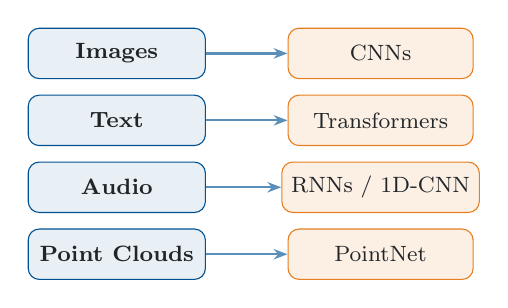
\begin{tikzpicture}[
        modbox/.style={rectangle, draw=UnifiBlue, fill=UnifiBlue!9,
                       rounded corners=4pt, minimum width=2.25cm, minimum height=0.64cm,
                       font=\footnotesize\bfseries, text=UnifiDark},
        archbox/.style={rectangle, draw=AccentOrange, fill=AccentOrange!12,
                        rounded corners=4pt, minimum width=2.35cm, minimum height=0.64cm,
                        font=\footnotesize, text=UnifiDark},
        myarrow/.style={-{Stealth[length=5pt]}, thick, UnifiBlue!65}
      ]
        \node[modbox] (img) at (0,0) {Images};
        \node[modbox] (txt) at (0,-0.85) {Text};
        \node[modbox] (aud) at (0,-1.70) {Audio};
        \node[modbox] (pc)  at (0,-2.55) {Point Clouds};

        \node[archbox] (cnn)   at (3.35,0) {CNNs};
        \node[archbox] (trans) at (3.35,-0.85) {Transformers};
        \node[archbox] (rnn)   at (3.35,-1.70) {RNNs / 1D-CNN};
        \node[archbox] (pnet)  at (3.35,-2.55) {PointNet};

        \draw[myarrow] (img) -- (cnn);
        \draw[myarrow] (txt) -- (trans);
        \draw[myarrow] (aud) -- (rnn);
        \draw[myarrow] (pc)  -- (pnet);
      \end{tikzpicture}
      \end{center}

      \vspace{0.35em}
      \small
      Each data type is usually paired with a dedicated model and
      domain-specific assumptions about structure.
    \end{column}

    \begin{column}{0.40\textwidth}
      {\color{UnifiBlue}\large\bfseries The scaling bottleneck}

      \vspace{0.45em}
      \colhead{Self-attention cost}
        \centering
        {\Large $\mathcal{O}(M^2 \cdot d)$}\\[0.2em]
        {\scriptsize grows quadratically with input length $M$}
      

      \vspace{0.35em}
      \begin{table}
        \centering\small
        \begin{tabular}{lr}
          \toprule
          \textbf{Input representation} & \textbf{$M$} \\
          \midrule
          $16\!\times\!16$ image patches & $256$ \\
          raw $224\!\times\!224$ pixels & $50{,}176$ \\
          \bottomrule
        \end{tabular}
      \end{table}

      \vspace{0.15em}
      \centering\small
      Raw pixels make standard attention \alert{impractical}.
    \end{column}
  \end{columns}

  \vspace{1.1em}
  {\color{UnifiBlue!25}\hrule height 0.6pt}
  \vspace{0.6em}
  \centering\small
  {\color{UnifiBlue}\textbf{Core question:}}\, can one architecture handle arbitrary inputs without quadratic cost?
\end{frame}

\newcommand{\SolutionCard}[3]{%
  \begin{beamercolorbox}[wd=\linewidth,rounded=true,shadow=true,sep=0pt]{solution card body}
    \begin{beamercolorbox}[wd=\linewidth,rounded=true,sep=0.06cm,leftskip=0.16cm]{solution card title}
      {\normalsize #1}
    \end{beamercolorbox}
    \vspace{0.10em}
    \hspace{0.16cm}\begin{minipage}[t][0.74cm][t]{0.88\linewidth}
      \raggedright
      \hyphenpenalty=10000\exhyphenpenalty=10000
      {\scriptsize\bfseries #2}\\[-0.10em]
      {\scriptsize #3}
    \end{minipage}
    \vspace{0.10em}
  \end{beamercolorbox}%
}

% ── Slide 4: The Perceiver Solution ─────────────────────────────────────────────
\begin{frame}[shrink=5]{The Perceiver Solution}
  \setbeamercolor{solution card title}{bg=UnifiBlue, fg=white}
  \setbeamercolor{solution card body}{bg=UnifiBlue!8, fg=UnifiDark}
  \small
  \begin{center}
    \begin{minipage}{0.88\textwidth}
      \centering
      {\color{UnifiBlue}\textbf{Core idea:}} learned latents read the input once; expensive processing stays in latent space.
    \end{minipage}
  \end{center}

  \vspace{0.80em}
  \noindent
  \begin{minipage}[t]{0.29\textwidth}
    \SolutionCard{1. Read}{Cross-attention}{$M$ inputs $\to$ $N \ll M$ latents}
  \end{minipage}\hfill
  \begin{minipage}[t]{0.29\textwidth}
    \SolutionCard{2. Process}{Latent block}{transform $N$ latent slots}
  \end{minipage}\hfill
  \begin{minipage}[t]{0.29\textwidth}
    \SolutionCard{3. Reuse}{Shared weights}{repeat the same processor}
  \end{minipage}

  \vspace{0.22em}
  \begin{center}
    {\color{UnifiDark}\bfseries Complexity shift}

    \vspace{0.18em}
    {\footnotesize Read the full input once; repeat the expensive work in the compact latent space $N \ll M$.}

    \vspace{0.24em}
    \scriptsize
    \renewcommand{\arraystretch}{1.04}
    \begin{tabular*}{0.66\textwidth}{@{\extracolsep{\fill}}lc}
      \toprule
      \textbf{Operation} & \textbf{Cost} \\
      \midrule
      Read input once & $\mathcal{O}(M \cdot N)$ \\
      Process latents for $L$ layers & $\mathcal{O}(L \cdot N^2)$ \\
      \midrule
      \textbf{Perceiver} & $\mathcal{O}(M N + L N^2)$ \\
      \bottomrule
    \end{tabular*}
  \end{center}
\end{frame}

% ── Slide 5: Perceiver IO ───────────────────────────────────────────────────────
\section{Perceiver}

\begin{frame}[shrink=5]{Perceiver Architecture}
  \begin{center}
    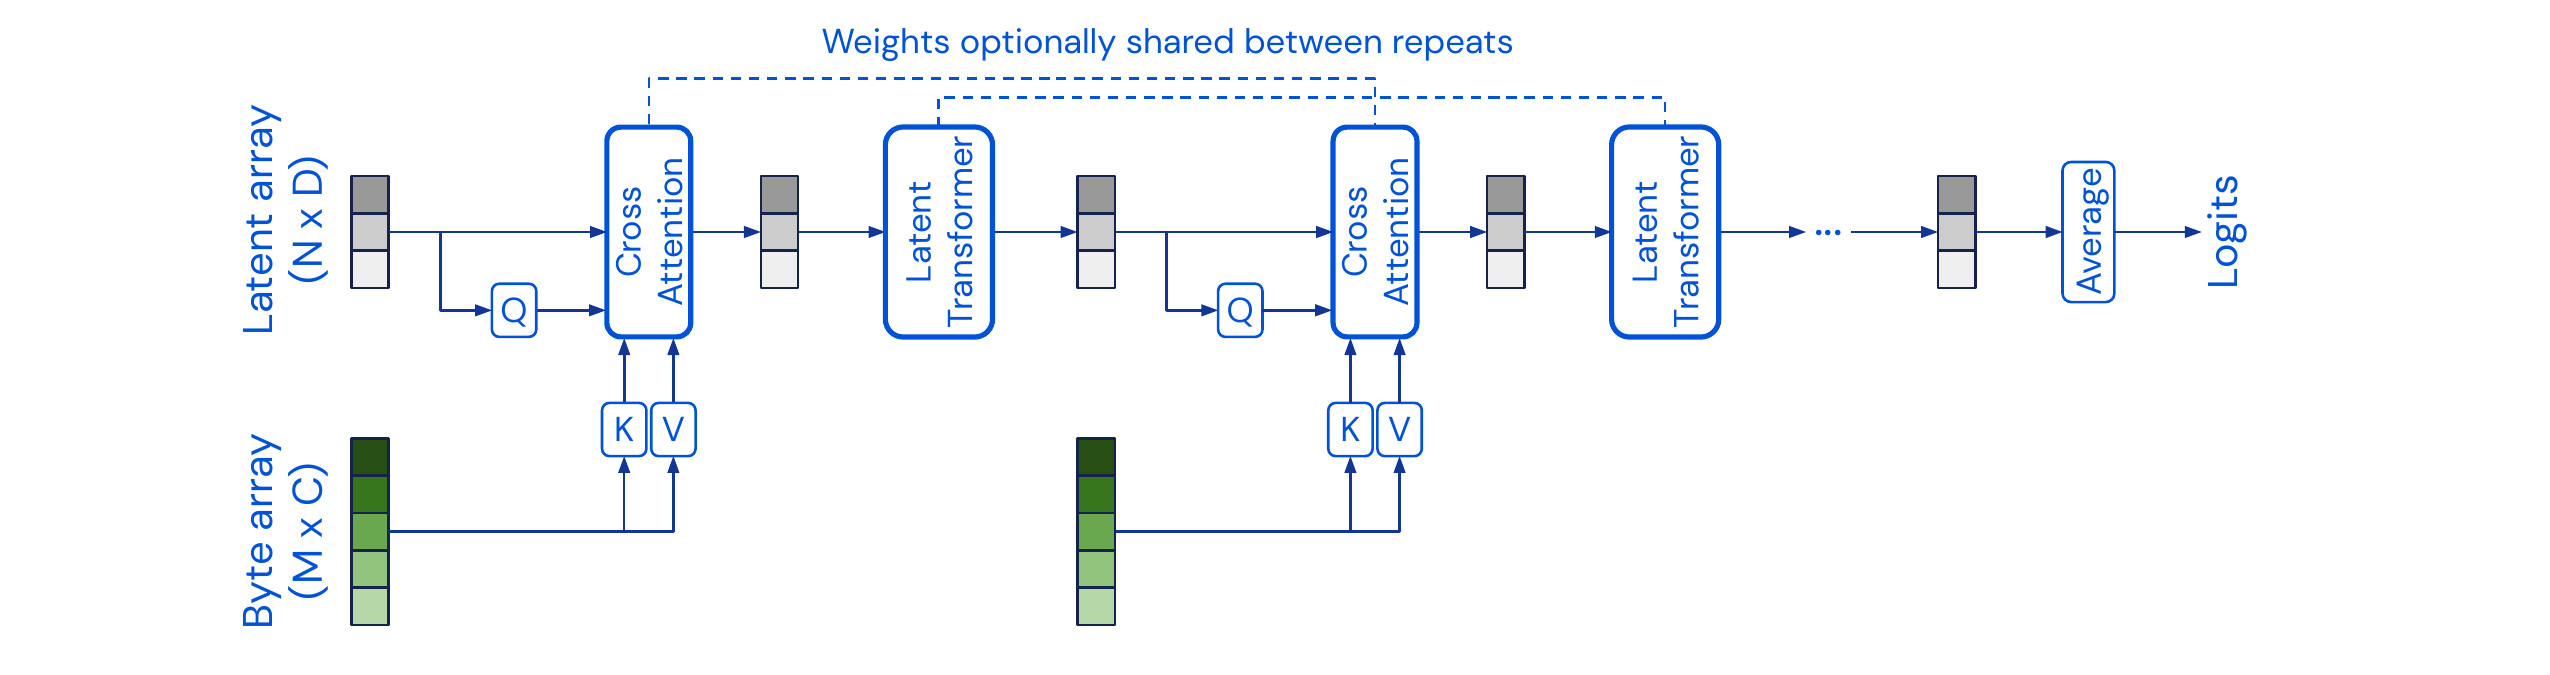
\includegraphics[width=0.98\textwidth,height=0.39\textheight,keepaspectratio]{perceiver_arch.png}
  \end{center}

  \vspace{0em}
  \small
  \begin{columns}[T,onlytextwidth]
    \begin{column}{0.50\textwidth}
      \textbf{Encode and process}
      \begin{itemize}
        \item $X \in \mathbb{R}^{M \times C}$ supplies keys and values.
        \item $Z \in \mathbb{R}^{N \times D}$ supplies queries, with $N \ll M$.
        \item Cross-attention maps $X \rightarrow Z$: $\mathcal{O}(M N)$.
      \end{itemize}
    \end{column}

    \begin{column}{0.46\textwidth}
      \textbf{Latent core and output}
      \begin{itemize}
        \item Latent Transformer updates $Z$ only.
        \item Repeated blocks may share weights.
        \item Original Perceiver pools $Z$; Perceiver IO uses output queries.
      \end{itemize}
    \end{column}
  \end{columns}
\end{frame}

% ══════════════════════════════════════════════════════════════════════════════
% SECTION 2: Architecture (slides 5-13)
% ══════════════════════════════════════════════════════════════════════════════
% Section marker moved before the merged architecture slide.

% ── Slide 6: Architecture Overview ──────────────────────────────────────────────
% ── Slide 7: Cross-Attention ────────────────────────────────────────────────────
\begin{frame}{Cross-Attention: The Key Mechanism}
  \begin{columns}[T]
    \begin{column}{0.48\textwidth}
      \textbf{Formally:}
      \begin{align*}
        Q &= Z \, W_Q \in \mathbb{R}^{N \times d_k} \\
        K &= X \, W_K \in \mathbb{R}^{M \times d_k} \\
        V &= X \, W_V \in \mathbb{R}^{M \times d_k}
      \end{align*}
      \[
      \text{CrossAttn}(Q,K,V) = \text{softmax}\!\left(\frac{QK^\top}{\sqrt{d_k}}\right) V
      \]

      \vspace{0.3em}
      The \alert{latents $Z$ are the queries}, the input $X$ provides keys and values $\Rightarrow$ informational \textit{bottleneck}.
    \end{column}
    \begin{column}{0.48\textwidth}
      \begin{center}
        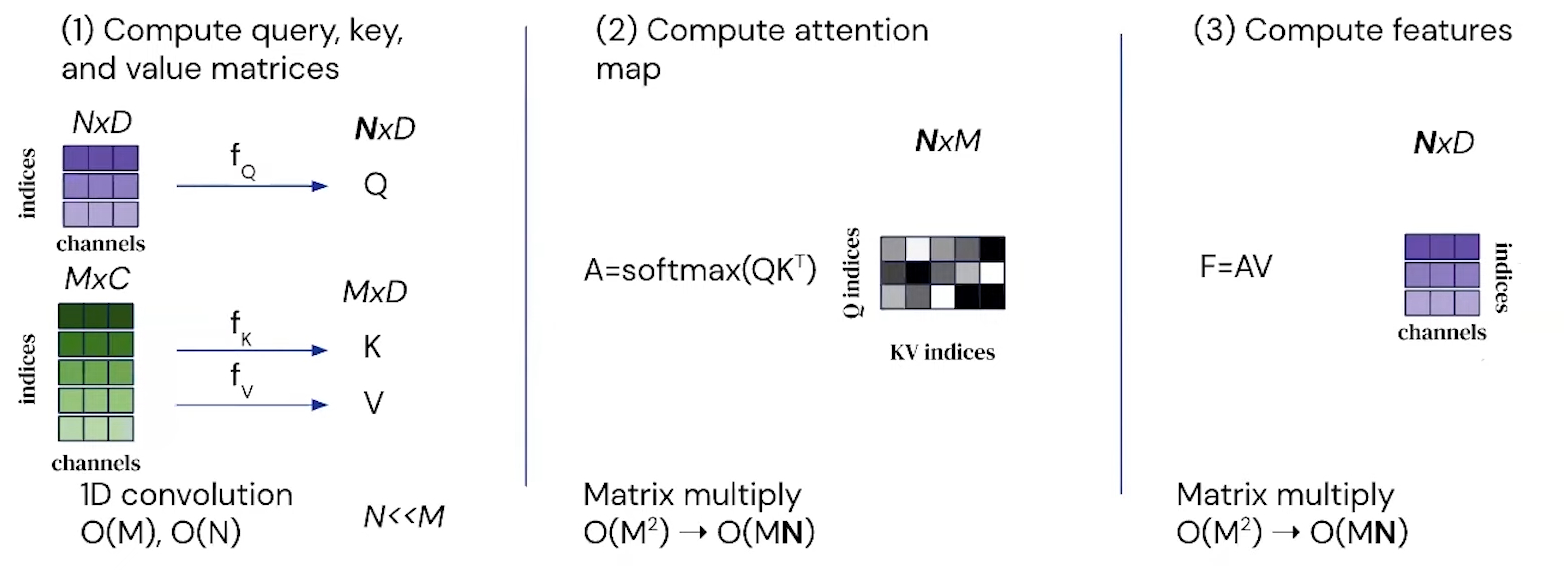
\includegraphics[width=\textwidth,height=0.33\textheight,keepaspectratio]{cross_attention_steps.png}
      \end{center}

      \vspace{0.3em}
      \textbf{Key insight:}
      \begin{itemize}
        \item Attention matrix: $N \times M$ (not $M \times M$)
        \item Complexity: $\mathcal{O}(N \cdot M \cdot d_k)$
        \item Decouples depth from input size
      \end{itemize}
    \end{column}
  \end{columns}
\end{frame}

% ── Slide 8: Latent Transformer & Weight Sharing ────────────────────────────────
\begin{frame}[shrink=3]{Latent Transformer \& Weight Sharing}
  \small
  \textbf{Once information is in the latent array, depth is spent by reusing the same processor on a compact state.}

  \vspace{0.4em}
  \begin{center}
    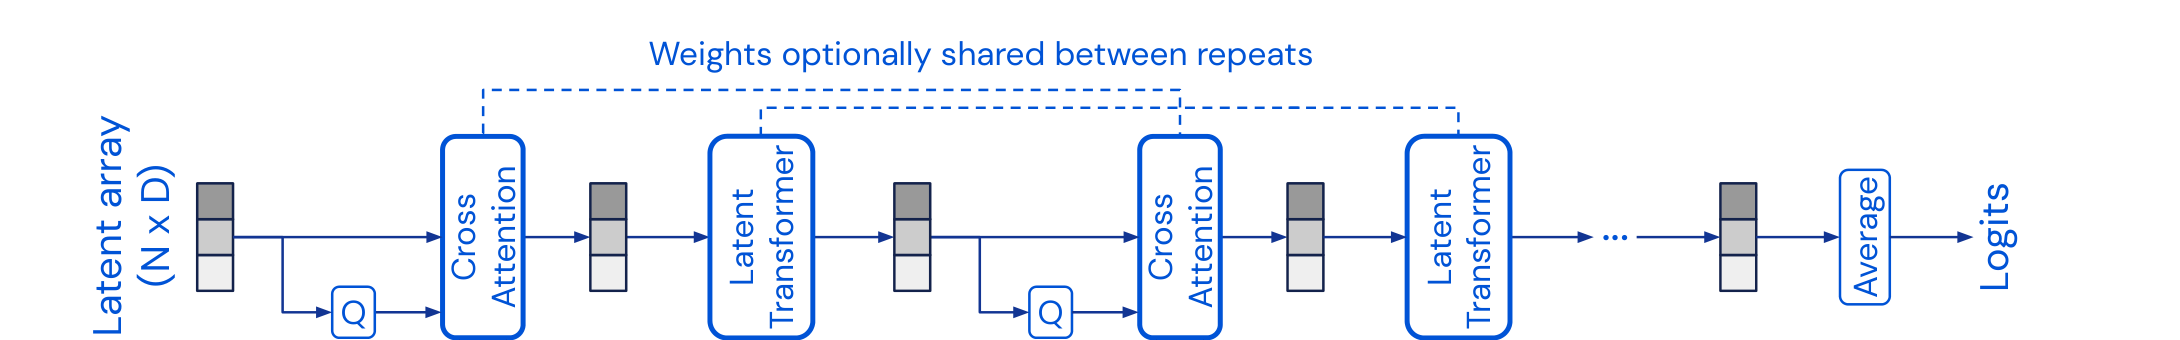
\includegraphics[width=0.97\textwidth,height=0.42\textheight,keepaspectratio]{perceiver_architecture_overview.png}
  \end{center}

  \vspace{0.5em}
  \begin{columns}[T,onlytextwidth]
    \begin{column}{0.48\textwidth}
      \textbf{Weight sharing}
      \begin{itemize}
        \item The same Latent Transformer block $B_{\theta}$ is reused at every repeat, with shared parameters $\theta$.
        \item Unrolling depth behaves like an RNN over the latent state:
          $Z_{t+1}=B_{\theta}(Z_t)$.
      \end{itemize}
    \end{column}

    \begin{column}{0.48\textwidth}
      \textbf{Why it matters}
      \begin{itemize}
        \item Iterative refinement without instantiating a new processor at each step.
        \item Parameter count stays fixed as depth grows; computation stays in the $N$-slot latent space.
      \end{itemize}
    \end{column}
  \end{columns}
\end{frame}

% ── Slide 9: Fourier Positional Encoding ────────────────────────────────────────
\begin{frame}[shrink=9]{Fourier Positional Encoding}
  \small
  \textbf{Perceiver receives a flat array, so location has to be part of each input token.}

  \vspace{0.2em}
  \begin{center}
    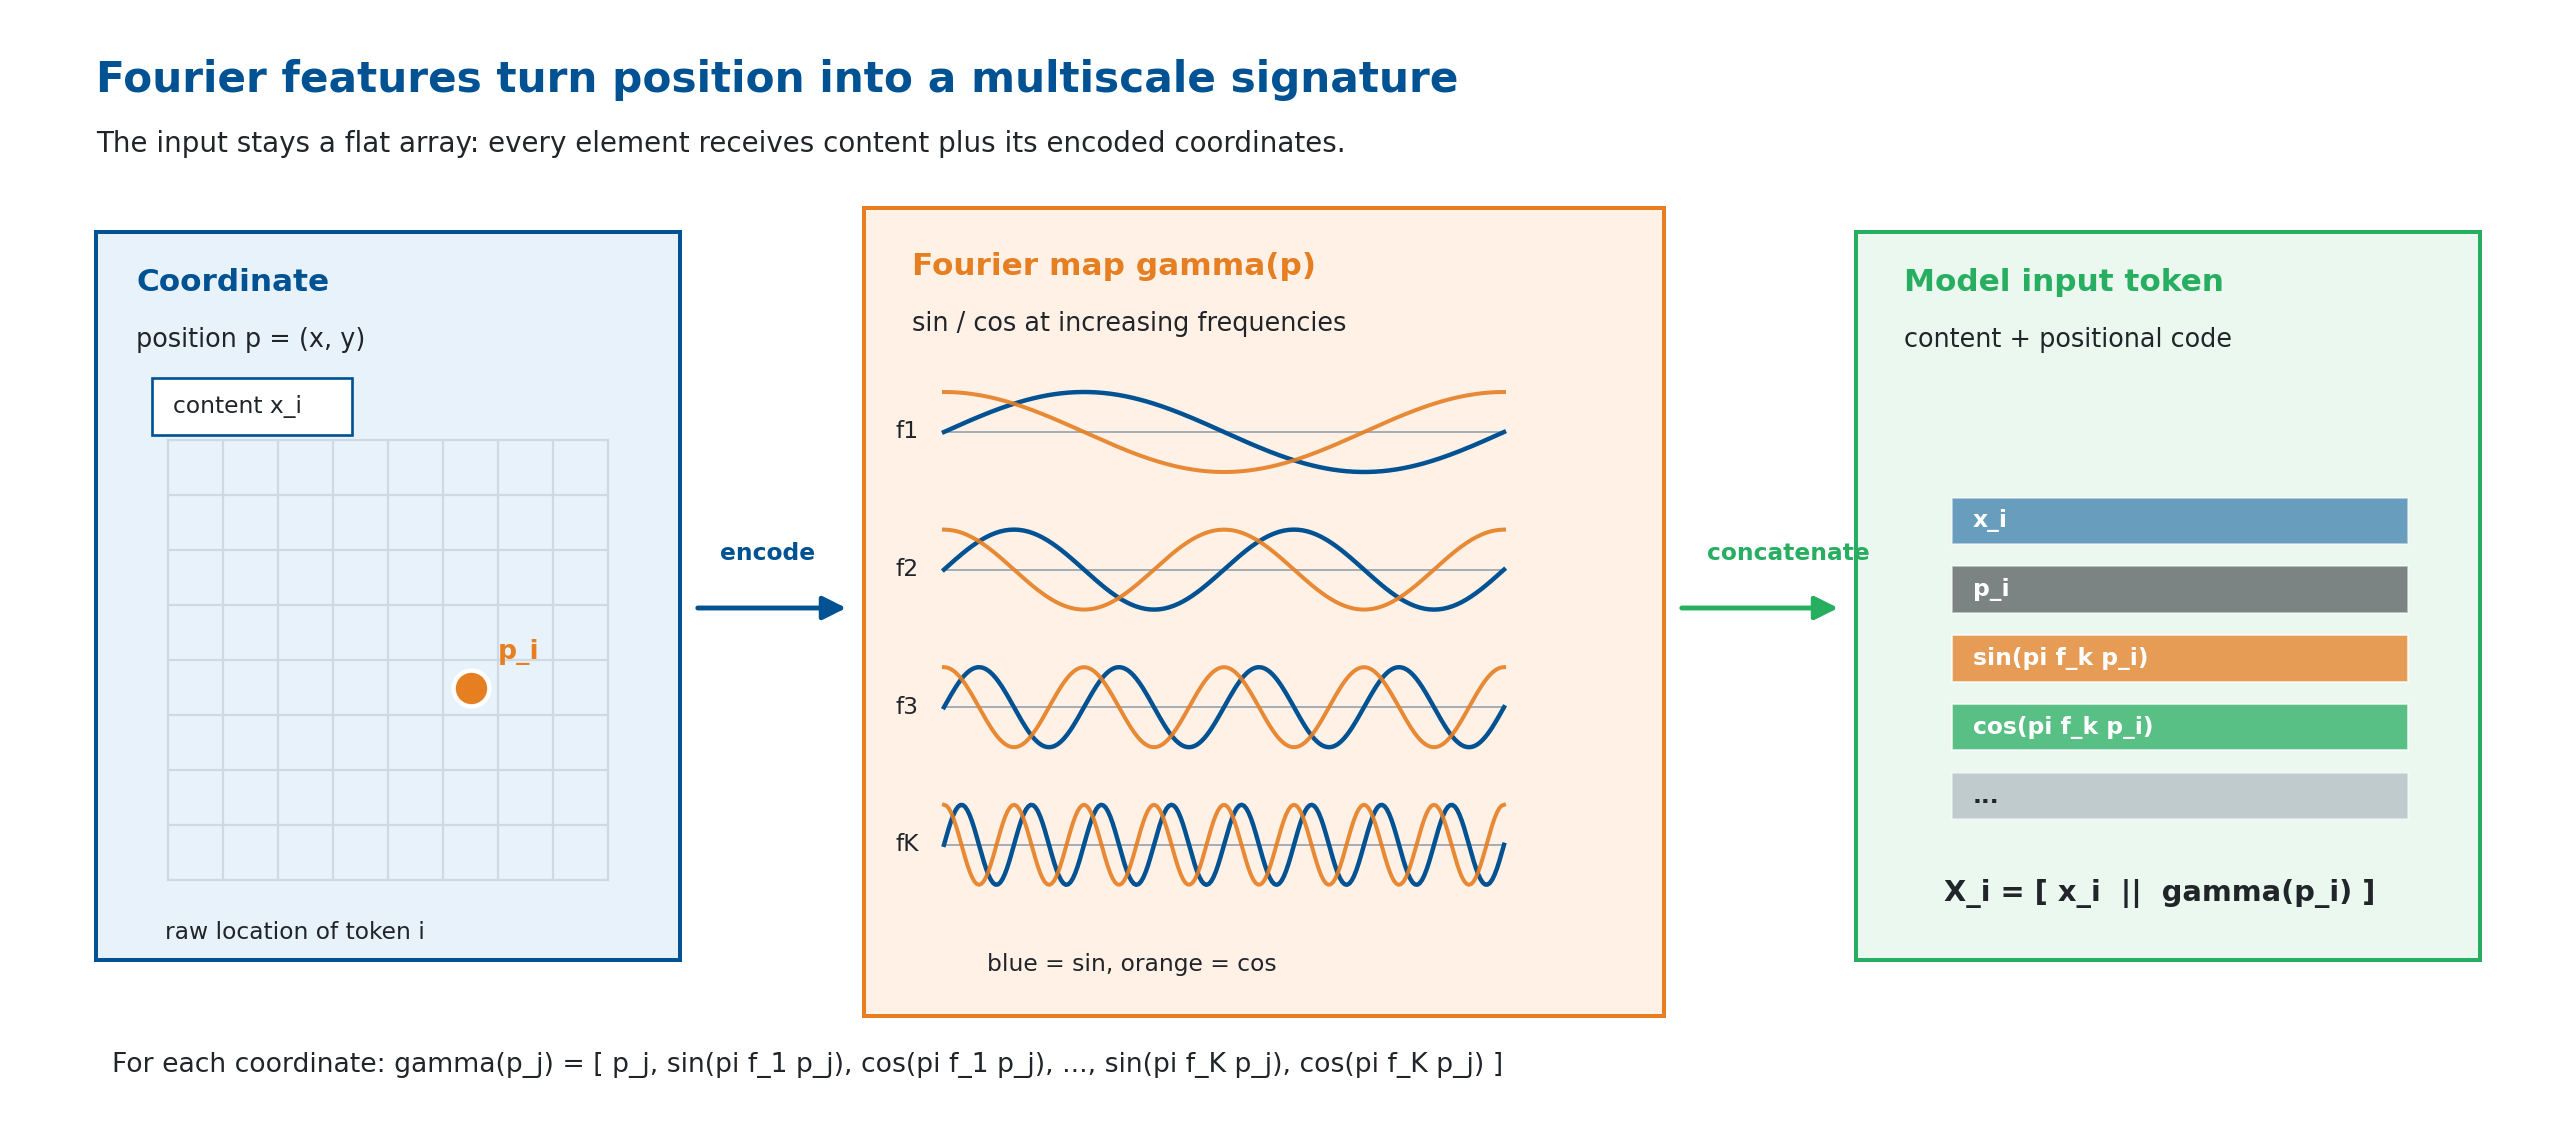
\includegraphics[width=1.0\textwidth,height=0.53\textheight,keepaspectratio]{fourier_features_encoding.png}
  \end{center}

  \vspace{0.35em}
  \begin{columns}[T,onlytextwidth]
    \begin{column}{0.49\textwidth}
      \textbf{General recipe}
      \par\smallskip
      Use domain coordinates: images $(u,v)$, point clouds $(x,y,z)$,
      or text index $t$; sine/cosine bands encode them at multiple scales.
    \end{column}

    \begin{column}{0.47\textwidth}
      \textbf{Input seen by attention}
      \par\smallskip
      The array is still flat, but each token is enriched before projection:
      $X_i=[\,x_i\,\|\,\gamma(p_i)\,]$.
    \end{column}
  \end{columns}
\end{frame}

% ── Slide 10: Perceiver IO Decoder ──────────────────────────────────────────────
\begin{frame}[shrink=8]{Perceiver Forward Pass: Shape Checkpoints}
  \begin{columns}[T]
    \begin{column}{0.52\textwidth}
      \textbf{Data flow in the original Perceiver:}
      \begin{enumerate}
        \item Input array: each token stacks content $\mathbf{x}$ with a Fourier position code $\gamma(\mathbf{p})$,
        \[
          X=[\,\mathbf{x}\,\|\,\gamma(\mathbf{p})\,]\in\mathbb{R}^{M\times C}.
        \]
        \item Learned latent array:
        \[
          Z_0\in\mathbb{R}^{N\times D},\qquad N\ll M
        \]
        \item Cross-attention reads input:
        \[
          Q=ZW_Q,\quad K=XW_K,\quad V=XW_V
        \]
        \item Latent Transformer applies self-attention + FFN only on $N$ latents.
      \end{enumerate}
    \end{column}
    \begin{column}{0.44\textwidth}
      \textbf{Shape checkpoints:}
      \begin{table}
        \centering\scriptsize
        \begin{tabular}{lll}
          \toprule
          \textbf{Object} & \textbf{Shape} & \textbf{Meaning} \\
          \midrule
          $X$ & $M\times C$ & input array (content+pos) \\
          $Z_0$ & $N\times D$ & learned latents \\
          $Q$ & $N\times d_k$ & latent queries \\
          $K,V$ & $M\times d_k$ & input keys/values \\
          $A$ & $N\times M$ & attention map \\
          \bottomrule
        \end{tabular}
      \end{table}

      \vspace{0.4em}
      \colhead{Core idea}
        The input size $M$ affects only the cross-attention read; depth is spent in the compact latent space.
      
    \end{column}
  \end{columns}
\end{frame}

% ── Slide 11: Output Query Design per Task ──────────────────────────────────────
\begin{frame}[shrink=5]{Original Perceiver Output: Pooling Classifier}
  \begin{columns}[T]
    \begin{column}{0.49\textwidth}
      \textbf{Fixed-shape output head:}
      \[
        Z_T=\mathrm{Encoder}(X,Z_0)
      \]
      \[
        z=\frac{1}{N}\sum_{i=1}^{N}Z_T[i]
      \]
      \[
        \mathrm{logits}=zW_{\mathrm{cls}}+b_{\mathrm{cls}}
      \]

      \vspace{0.4em}
      \begin{itemize}
        \item Mean pooling collapses all latents to one vector
        \item The classifier predicts one global label
        \item This is ideal for classification, not dense structured outputs
      \end{itemize}
    \end{column}
    \begin{column}{0.47\textwidth}
      \small
      \textbf{Where FFN and sharing fit:}
      \begin{itemize}
        \item Each latent block is pre-norm attention, residual, FFN, residual
        \item FFN adds non-linearity after attention mixing
        \item Weight sharing repeats the processor over iterations
      \end{itemize}

      \vspace{0.35em}
      \colhead{Fixed-shape output}
        Pooling collapses the $N$ latents into a single vector, so this head emits one global prediction per input.
      
    \end{column}
  \end{columns}
\end{frame}

% ── Slide 12: Computational Complexity ──────────────────────────────────────────
\begin{frame}[shrink=5]{Computational Complexity Analysis}
  \small
  \begin{table}
    \centering\small
    \begin{tabular}{lccc}
      \toprule
      \textbf{Model} & \textbf{Self-Attn} & \textbf{Cross-Attn} & \textbf{Total} \\
      \midrule
      Standard Transformer & $\mathcal{O}(M^2 d)$ & --- & $\mathcal{O}(M^2 d \cdot L)$ \\
      \midrule
      Perceiver & $\mathcal{O}(N^2 d)$ & $\mathcal{O}(MNd)$ & $\mathcal{O}((MN + N^2 L)\,d)$ \\
      \bottomrule
    \end{tabular}
  \end{table}

  \vspace{0.5em}
  \begin{columns}[T]
    \begin{column}{0.48\textwidth}
      \textbf{Symbols:}
      \begin{itemize}
        \item $M$: number of input elements
        \item $N$: number of latent slots, with $N \ll M$
        \item $L$: number of latent processing layers
        \item $d$: hidden channel dimension
      \end{itemize}
    \end{column}
    \begin{column}{0.48\textwidth}
      \textbf{Interpretation:}
      \begin{itemize}
        \item The full input is read through cross-attention
        \item Repeated self-attention happens only in latent space
        \item If $N$ is fixed, depth becomes independent of input length
        \item Concrete sizes are evaluated in the experiments
      \end{itemize}
    \end{column}
  \end{columns}
\end{frame}

% ── Slide 13: GELU & LAMB Optimizer ─────────────────────────────────────────────
\section{Experiments: Perceiver}

\begin{frame}[shrink=5]{GELU Activation \& LAMB Optimizer}
  \begin{columns}[T,onlytextwidth]
    \begin{column}{0.48\textwidth}
      \small
      \textbf{GELU (Gaussian Error Linear Unit):}
      \[
      \text{GELU}(x) = x \cdot \Phi(x) \approx x \cdot \sigma(1.702\,x)
      \]
      \vspace{-0.25em}
      \begin{itemize}
        \item Smooth activation used in Transformer architectures
        \item Allows small negative gradient flow
      \end{itemize}

      \vspace{0.2em}
      \textbf{LAMB (Layer-wise Adaptive Moments):}
      \vspace{-0.25em}
      \[
      r_t^{(l)} = \frac{\|w_t^{(l)}\|}{\|w_t^{(l)} + \eta\, \hat{u}_t^{(l)}\|}
      \]
      \vspace{-0.55em}
      {\footnotesize Per-layer trust ratio rescales updates and stabilizes large-batch training.}
    \end{column}
    \begin{column}{0.48\textwidth}
      \small
      \textbf{Why LAMB for Perceiver?}
      \begin{itemize}
        \item Cross-attention bottleneck creates high variance gradients
        \item Standard Adam can \alert{destabilize} with large batches
        \item LAMB safely scales batch sizes up to 1024
      \end{itemize}

      \vspace{0.25em}
      \begin{table}
        \centering\scriptsize
        \begin{tabular}{lcc}
          \toprule
          \textbf{Optimizer} & \textbf{Large Batches} & \textbf{Layer-wise LR} \\
          \midrule
          Adam & Diverges & Global \\
          \textbf{LAMB} & \textbf{Stable} & \textbf{Per-layer trust} \\
          \bottomrule
        \end{tabular}
      \end{table}
    \end{column}
  \end{columns}
\end{frame}

% ── Slide 14: Implementation ────────────────────────────────────────────────────
\begin{frame}[shrink=5]{Implementation}
  \vspace{0.15em}
  \begin{table}
    \centering\scriptsize
    \begin{tabular}{>{\raggedright\arraybackslash}p{0.18\textwidth}>{\raggedright\arraybackslash}p{0.36\textwidth}>{\raggedright\arraybackslash}p{0.36\textwidth}}
      \toprule
      \textbf{Aspect} & \textbf{Paper implementation} & \textbf{Project code} \\
      \midrule
      Core model &
      Cross-attention into learned latents, latent self-attention, FFN, weight sharing &
      Same modules; weight sharing is exposed as an ablation switch \\
      \midrule
      Model scale &
      Large vision/language runs: up to $512{\times}1024$ latents and 201M-param IO &
      Smaller runs: CIFAR-10 $96{\times}384$, ModelNet40/text $128{\times}512$ \\
      \midrule
      Data setting &
      ImageNet, ModelNet40, large language pretraining corpora &
      CIFAR-10, ModelNet40, WikiText-103 byte-level MLM, GLUE fine-tuning \\
      \midrule
      Training budget &
      Distributed accelerators, batches up to 512--1024 &
      Single-GPU budget, batches 32--64, LAMB retained for stability \\
      \midrule
      Practical additions &
      Minimal regularization in the reference setup &
      Validation split carved from train, fixed seed, attention-map extraction, declarative run registry \\
      \bottomrule
    \end{tabular}
  \end{table}

  \vspace{0.25em}
  {\small The implementation keeps the architectural mechanism intact; the main differences are scale, data budget and training resources.}
\end{frame}

% -- Slide 14b: Implementation Differences from the Paper --
\begin{frame}[shrink=11]{Implementation Differences from the Paper}
  \vspace{0.15em}
  \begin{table}
    \centering\scriptsize
    \begin{tabular}{>{\raggedright\arraybackslash}p{0.20\textwidth}>{\raggedright\arraybackslash}p{0.34\textwidth}>{\raggedright\arraybackslash}p{0.38\textwidth}}
      \toprule
      \textbf{Choice} & \textbf{Original paper (ImageNet)} & \textbf{This project} \\
      \midrule
      Input tokenization &
      Raw pixels, no patching ($M=50{,}176$) &
      \textbf{Raw pixels, no patching} ($M=1{,}024$ on $32{\times}32$) \\
      \addlinespace[2pt]
      Latent array $N\times D$ &
      $512\times1024$ &
      $96\times384$ (CIFAR-10), $128\times512$ (ModelNet40) \\
      \addlinespace[2pt]
      Cross-attend iterations $T$ &
      $8$ &
      $4$ (CIFAR-10), $2$ (ModelNet40) --- and $T$ is itself an ablation axis \\
      \addlinespace[2pt]
      Positional encoding &
      2D Fourier, $K=64$ bands/axis ($258$ dims) &
      \textbf{Identical}: 2D Fourier, $K=64$ bands/axis, $258$ dims $+$ 3 RGB $=261$ \\
      \addlinespace[2pt]
      Weight sharing &
      On by default (shared across $T$) &
      Exposed as an ablation switch (on/off) \\
      \addlinespace[2pt]
      Model selection &
      --- &
      \textbf{Validation carved from train} (45k/5k/10k); test touched once \\
      \addlinespace[2pt]
      Parameters &
      $30$--$200\text{M}+$ &
      $10.18$M (CIFAR-10), $23.29$M (ModelNet40), $18.87$M (IO text) \\
      \bottomrule
    \end{tabular}
  \end{table}

  \vspace{0.3em}
  \colhead{Kept identical to the paper}
    \small Core mechanism preserved: cross-attention bottleneck $\to$ weight-shared latent transformer $\to$ mean-pooling (Perceiver) / output-query decoder (IO); GELU MLP, pre-norm LayerNorm, Fourier frequencies linearly spaced to Nyquist.
  
\end{frame}

% ══════════════════════════════════════════════════════════════════════════════
% SECTION 3: Experiments & Results (slides 15-28)
% ══════════════════════════════════════════════════════════════════════════════


% ── Slide 15: CIFAR-10 Setup ────────────────────────────────────────────────────
\begin{frame}[shrink=11]{CIFAR-10: Experimental Setup}
  \textbf{Goal:} validate the Perceiver on raw pixels, with no convolutional assumption anywhere.

  \vspace{0.3em}
  \begin{columns}[T]
    \begin{column}{0.46\textwidth}
      \begin{table}
        \centering\small
        \begin{tabular}{ll}
          \toprule
          \textbf{Hyperparameter} & \textbf{Value} \\
          \midrule
          Latent array ($N \times D$) & $96 \times 384$ \\
          Cross-attn stages ($T$) & 4, interleaved \\
          Transformer blocks ($L$) & 4 (shared) \\
          Heads (cross / self) & 1 / 8 \\
          Fourier bands / max freq & 64 / 16 \\
          Dropout & 0 \\
          \midrule
          Optimizer & LAMB \\
          Learning rate & 0.004 \\
          Scheduler & MultiStep 84/102/114 \\
          Batch size & 64 \\
          Epochs & 120, \emph{no early stop} \\
          Precision & bfloat16 \\
          \midrule
          \textbf{Total parameters} & \textbf{10\,175\,362} \\
          \bottomrule
        \end{tabular}
      \end{table}
    \end{column}
    \begin{column}{0.50\textwidth}
      \colhead{Protocol --- the part that makes the numbers usable}
        \small
        Train split: \textbf{45\,000} images. Validation: \textbf{5\,000}, carved out of the training set. Test: the official \textbf{10\,000}, touched \emph{once}, at the very end.

        \vspace{0.4em}
        The reported checkpoint is the one with the best \emph{validation} accuracy. Selecting the epoch on the same set you report on is \textbf{selection leakage} and inflates every number.
      

      \vspace{0.4em}
      \textbf{Data pipeline}
      \begin{itemize}
        \item $32\!\times\!32$ RGB image $\to$ \textbf{1\,024 pixels} as an unordered set
        \item Each pixel: 3 RGB $+$ 2D Fourier PE $= $ \textbf{261 dims} --- the same per-pixel width as the paper
        \item No patching, no convolution, no learned tokenizer
      \end{itemize}
    \end{column}
  \end{columns}
\end{frame}

% ── The noise band ───────────────────────────────────────────────────────────
\begin{frame}[shrink=5]{The Noise Band: How Much Does a Number Move on Its Own?}
  \lead{Three runs, identical in everything but the seed, land 2.78 points apart. Read every other comparison against that.}
  \begin{columns}[T]
    \begin{column}{0.52\textwidth}
      \textbf{Three runs, identical in everything but the seed:}
      \begin{table}
        \centering\small
        \begin{tabular}{llc}
          \toprule
          \textbf{Run} & \textbf{Seed} & \textbf{Test acc.} \\
          \midrule
          \texttt{e01\_baseline} & 42 & 71.63\% \\
          \texttt{e31\_baseline\_seed1} & 1 & 68.85\% \\
          \texttt{e32\_baseline\_seed2} & 2 & 70.97\% \\
          \midrule
          \multicolumn{2}{l}{\textbf{Spread (max $-$ min)}} & \textbf{2.78pp} \\
          \bottomrule
        \end{tabular}
      \end{table}

      \vspace{0.3em}
      \alerthead{The rule for every slide that follows}
        \small
        Any difference smaller than \textbf{2.78 percentage points} is not an effect. It is seed variance.
      
    \end{column}
    \begin{column}{0.44\textwidth}
      \colhead{Why this slide exists}
        \small
        Two extra runs cost a few GPU-hours and change the status of all the others: without a measured band, every comparison is an opinion.

        \vspace{0.4em}
        It also sets the honest ceiling of this study. On CIFAR-10 with 1\,024 pixels and one GPU, most of the paper's ablations --- measured on ImageNet with 50\,176 pixels and 64 TPUs --- simply do not have room to show up.
      

      \vspace{0.3em}
      \scriptsize The band depends on the metric: 2.78pp on test accuracy, 2.94pp on best validation, 3.24pp on final validation. The conclusions do not change.
    \end{column}
  \end{columns}
\end{frame}

% ── Ablation overview ────────────────────────────────────────────────────────
\begin{frame}[shrink=12]{CIFAR-10: What Survives the Noise Band}
  \lead{Ranked against the band: twelve of the twenty-four runs clear it, the other twelve are inconclusive.}
  \begin{columns}[T,onlytextwidth]
    \begin{column}{0.70\textwidth}
      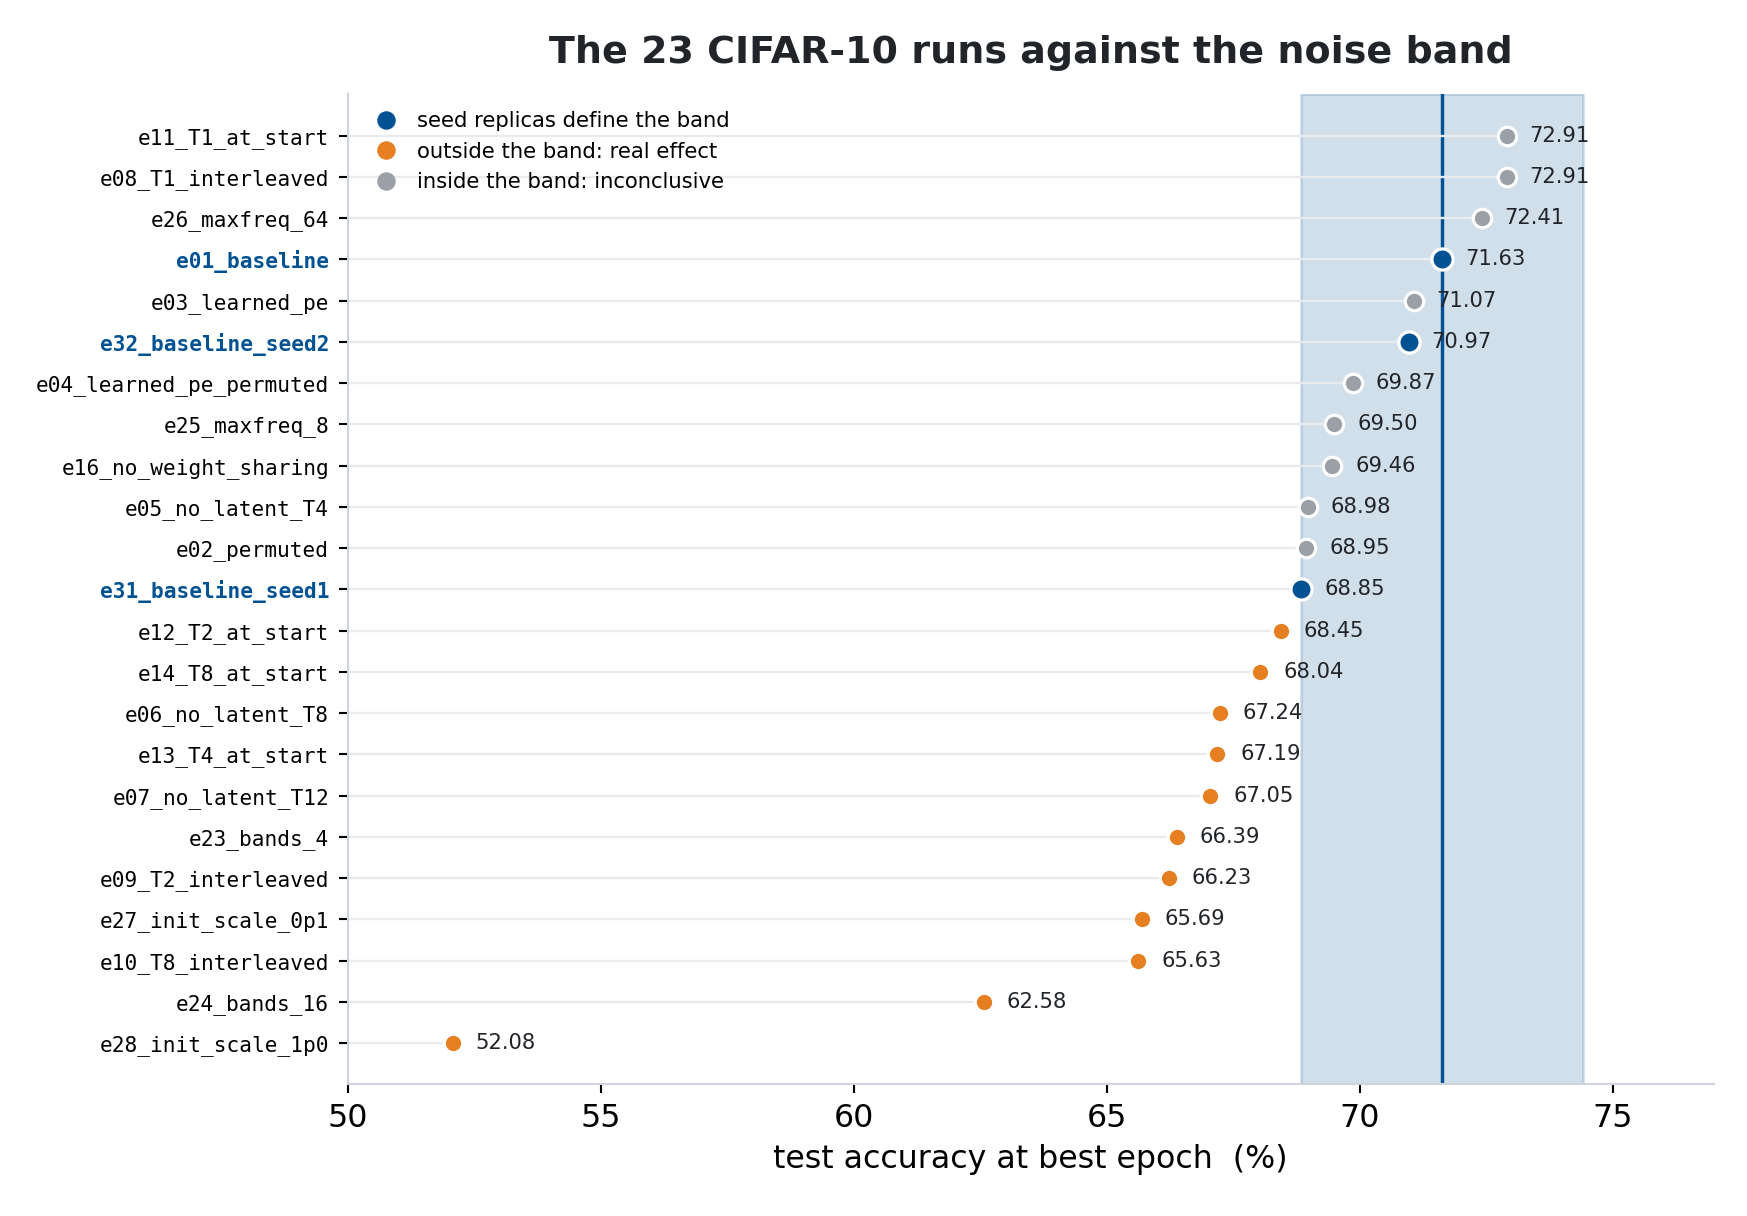
\includegraphics[width=\textwidth,height=0.74\textheight,keepaspectratio]{cifar10_ablation_correct.png}
    \end{column}
    \begin{column}{0.27\textwidth}
      \small
      \textbf{24 runs, 12 conclusive}

      \vspace{0.3em}
      \begin{itemize}
        \item \textcolor{AccentOrange}{\textbf{Outside}} the band: positional encoding, latent init scale, cross-attend arrangement, Fourier bands, no latent transformer
        \item \textcolor{gray}{\textbf{Inside}}: permutation, learned PE, weight sharing, max frequency
      \end{itemize}

      \vspace{0.2em}
      {\scriptsize The chart plots 23 runs: \texttt{e29\_no\_pe} at \textbf{32.36\%} is off scale. Source: each run's \texttt{results.json}, test accuracy at the validation-selected epoch.}
    \end{column}
  \end{columns}
\end{frame}

% ── Permutation ──────────────────────────────────────────────────────────────
\begin{frame}[shrink=11]{CIFAR-10: Permutation Invariance --- the Headline Claim}
  \lead{Shuffling the pixels costs nothing measurable. Removing the encoding costs 39.27 points. That contrast is the claim.}
  \begin{table}
    \centering\small
    \begin{tabular}{llcc}
      \toprule
      \textbf{Comparison} & \textbf{Positional encoding} & \textbf{Natural $\to$ permuted} & \textbf{$\Delta$} \\
      \midrule
      \texttt{e01} $\to$ \texttt{e02} & Fourier & $71.63\% \to 68.95\%$ & $-2.68$ \\
      \texttt{e03} $\to$ \texttt{e04} & learned & $71.07\% \to 69.87\%$ & $-1.20$ \\
      \midrule
      \texttt{e01} $\to$ \texttt{e29} & \alert{none at all} & $71.63\% \to 32.36\%$ & \textcolor{AccentRed}{$\mathbf{-39.27}$} \\
      \midrule
      \multicolumn{4}{l}{\textit{Paper (ImageNet):} Fourier $78.0 \to 78.0$ \quad learned $70.9 \to 70.9$} \\
      \bottomrule
    \end{tabular}
  \end{table}

  \vspace{0.4em}
  \begin{columns}[T]
    \begin{column}{0.48\textwidth}
      \colhead{What we measured}
        \small
        Both drops fall \textbf{inside} the 2.78pp band: shuffling the pixels causes no measurable damage. Invariance confirmed --- in the honest, weak form: \emph{we did not measure a loss}, which is not the same as proving the loss is zero.
      
    \end{column}
    \begin{column}{0.48\textwidth}
      \colhead{The control that makes it a claim}
        \small
        Shuffling the pixels costs nothing measurable; \textbf{removing the encoding costs 39.27pp}. The same architecture that ignores the order collapses without the coordinates. Position enters through the \textbf{encoding}, never through the grid --- and that contrast, not either number alone, is the evidence.
      
    \end{column}
  \end{columns}
\end{frame}

% ── Capacity ─────────────────────────────────────────────────────────────────
\begin{frame}[shrink=4]{CIFAR-10: Capacity Does Not Buy Accuracy}
  \lead{Three times the parameters do not buy a point: capacity is not what limits this model at CIFAR-10 scale.}
  \begin{columns}[T,onlytextwidth]
    \begin{column}{0.58\textwidth}
      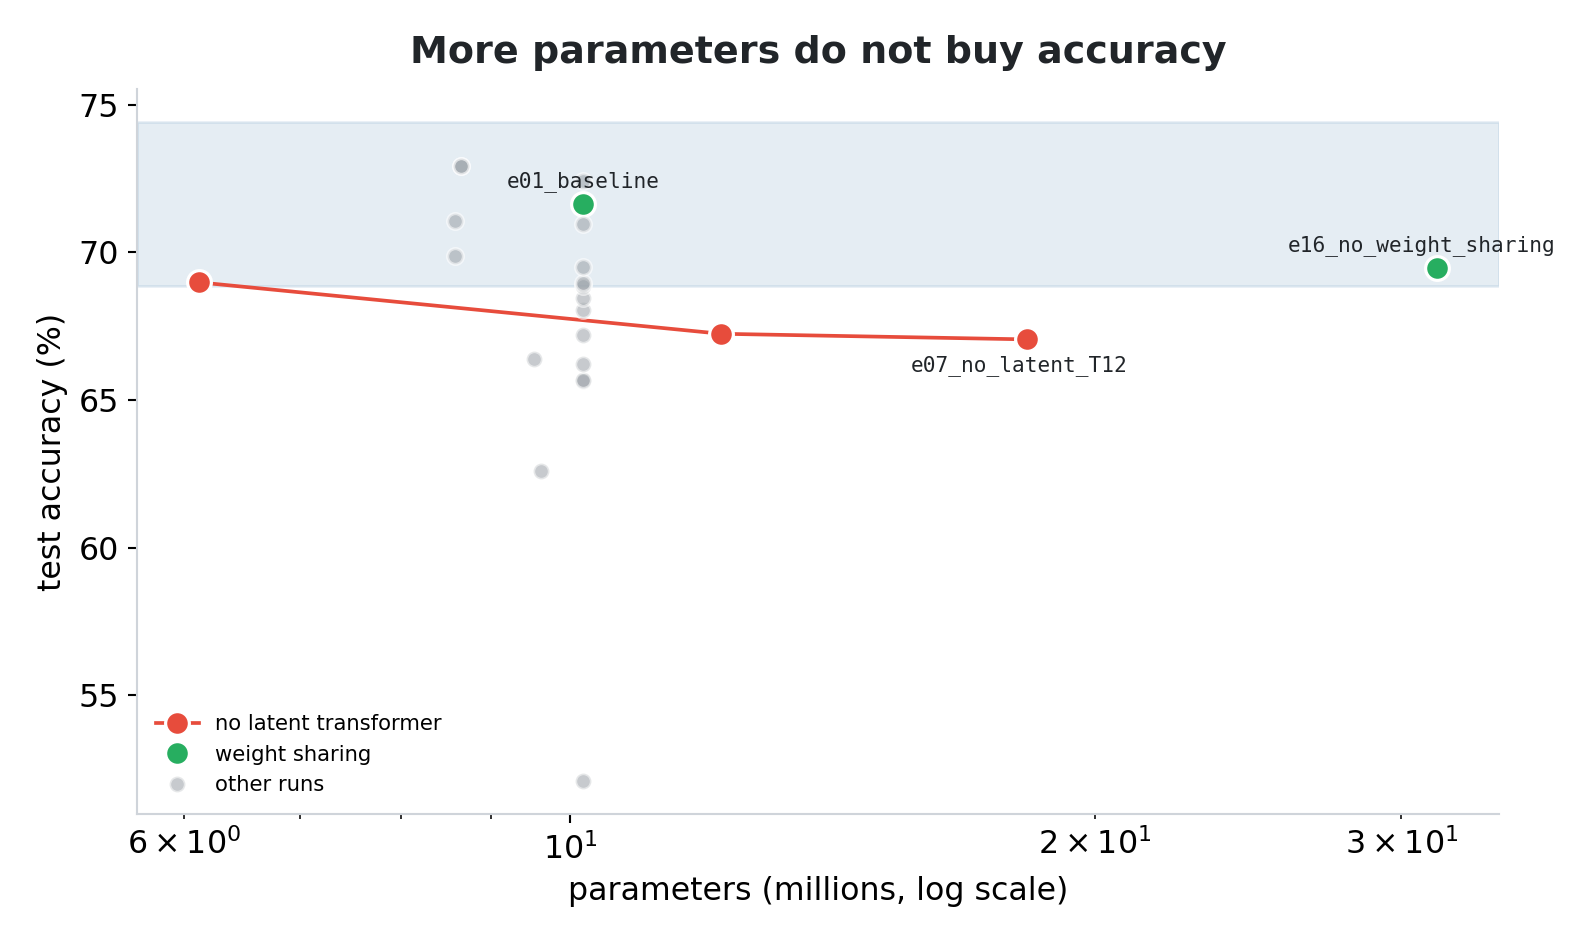
\includegraphics[width=\textwidth,height=0.66\textheight,keepaspectratio]{weight_sharing_tradeoff_correct.png}
    \end{column}
    \begin{column}{0.38\textwidth}
      \textbf{Weight sharing is free}
      \begin{itemize}\small
        \item \texttt{e01} 71.63\% with 10.2M params
        \item \texttt{e16} 69.46\% with \textbf{31.5M} params
        \item $3.1\times$ the weights, \textcolor{AccentRed}{$-$2.17pp} --- inside the band
      \end{itemize}

      \vspace{0.4em}
      \textbf{Where you put capacity matters}
      \begin{itemize}\small
        \item Remove the latent transformer, add cross-attends instead:
        \item 6.1M $\to$ 68.98\% \\ 12.2M $\to$ 67.24\% \\ 18.3M $\to$ 67.05\%
        \item \textcolor{AccentRed}{\textbf{More parameters, less accuracy}}
      \end{itemize}
    \end{column}
  \end{columns}
\end{frame}

% ── Tab. 6 ───────────────────────────────────────────────────────────────────
\begin{frame}[shrink=5]{CIFAR-10: How Many Cross-Attends, and Where}
  \begin{table}
    \centering\small
    \begin{tabular}{lccc}
      \toprule
      \textbf{$T$} & \textbf{interleaved} & \textbf{all at start} & \textbf{$\Delta$ (arrangement)} \\
      \midrule
      1 & \textbf{72.91\%} & \textbf{72.91\%} & $0.00$ \\
      2 & 66.23\% & 68.45\% & $+2.22$ \\
      4 & \textbf{71.63\%} \tiny(baseline) & 67.19\% & \textcolor{AccentRed}{$\mathbf{-4.44}$} \\
      8 & 65.63\% & 68.04\% & $+2.41$ \\
      \bottomrule
    \end{tabular}
  \end{table}

  \vspace{0.3em}
  \begin{columns}[T]
    \begin{column}{0.48\textwidth}
      \colhead{The one conclusive result}
        \small
        At $T=4$, interleaving beats front-loading by \textbf{4.44pp} --- outside the band. Re-reading the input \emph{after} the latents have been refined lets each pass look for something different.
      
    \end{column}
    \begin{column}{0.48\textwidth}
      \colhead{A reproducibility check, for free}
        \small
        At $T=1$ the two arrangements produce the \emph{same computational graph}, and indeed give bit-identical results: 72.91\%, epoch 90, 8\,654\,662 params. Fixed seed $\Rightarrow$ reproducible training.
      
    \end{column}
  \end{columns}

  \vspace{0.2em}
  \scriptsize Note the non-monotonicity along $T$: reading the input once is as good as reading it four times, with 15\% fewer parameters.
\end{frame}

% ── Fig. 6 ───────────────────────────────────────────────────────────────────
\begin{frame}[shrink=5]{CIFAR-10: The Hyperparameter That Actually Matters}
  \begin{columns}[T]
    \begin{column}{0.50\textwidth}
      \begin{table}
        \centering\small
        \begin{tabular}{lcc}
          \toprule
          \textbf{Sweep} & \textbf{Value} & \textbf{Test acc.} \\
          \midrule
          \multirow{3}{*}{Latent init $\sigma$}
            & \textbf{0.02} & \textbf{71.63\%} \\
            & 0.1 & \textcolor{AccentOrange}{65.69\%} \\
            & 1.0 & \textcolor{AccentRed}{\textbf{52.08\%}} \\
          \midrule
          \multirow{3}{*}{Fourier bands}
            & 4 & 66.39\% \\
            & 16 & 62.58\% \\
            & \textbf{64} & \textbf{71.63\%} \\
          \midrule
          \multirow{3}{*}{Max frequency}
            & 8 & 69.50\% \\
            & \textbf{16} & \textbf{71.63\%} \\
            & 64 & 72.41\% \\
          \bottomrule
        \end{tabular}
      \end{table}
    \end{column}
    \begin{column}{0.46\textwidth}
      \alerthead{Latent initialisation: the only clean monotone effect}
        \small
        $\sigma$ from 0.02 to 1.0 costs \textbf{19.55pp}. At $\sigma=1.0$ the best epoch is \textbf{9 out of 120}: the model learns briefly, then degrades for the remaining 111 epochs.
      

      \vspace{0.3em}
      \colhead{Two honest caveats}
        \scriptsize
        \textbf{Bands} is non-monotone (4 beats 16), and both low points are runs whose \emph{final} validation collapsed (22.5\% and 55.5\%) --- an optimisation problem, not a resolution one.

        \vspace{0.3em}
        \textbf{Max frequency} sits entirely inside the noise band. The whole axis is inconclusive, and saying so is part of the result.
      
    \end{column}
  \end{columns}
\end{frame}

% ── Baseline convoluzionale ──────────────────────────────────────────────────
\begin{frame}[shrink=14]{CIFAR-10: the Reference That Is Not a Perceiver}
  \lead{Neither Perceiver paper benchmarks CIFAR-10, so we trained the reference ourselves: a ResNet-18, same split, same epochs, same budget.}
  \begin{columns}[T,onlytextwidth]
    \begin{column}{0.48\textwidth}
      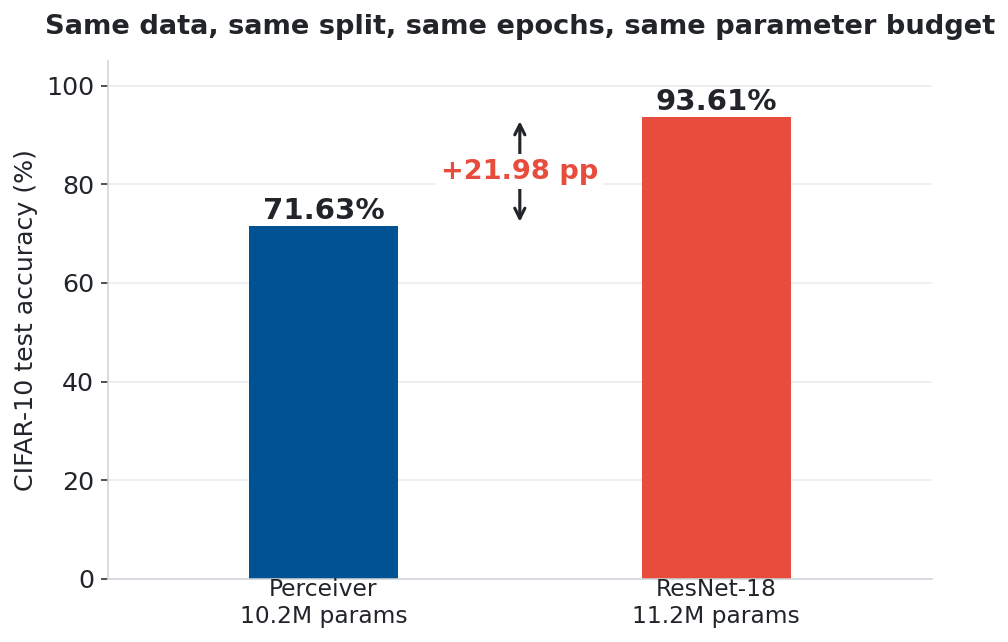
\includegraphics[width=\textwidth,height=0.60\textheight,keepaspectratio]{cnn_baseline_correct.png}
    \end{column}
    \begin{column}{0.48\textwidth}
      \alerthead{The uncomfortable comparison comes first}
        \small
        A \textbf{ResNet-18} on the same split, the same 120 epochs and 11.2M parameters against 10.2M reaches \textbf{93.61\%}, where \texttt{e01\_baseline} reaches \textbf{71.63\%}: \textcolor{AccentRed}{\textbf{$-$21.98pp}}.

        \vspace{0.3em}
        Neither Perceiver paper benchmarks CIFAR-10, so without this run there is nothing to read the number against.
      

      \vspace{0.3em}
      \colhead{What the gap actually measures}
        \small
        On ImageNet the paper \emph{beats} ResNet-50 by $+4.5$pp (78.0 vs 73.5). What differs between the two settings is not the architecture, it is the \textbf{scale}.

        \vspace{0.3em}
        The Perceiver's claim was never accuracy --- it is \alert{having no prior on the domain}. Here that prior is worth 22 points.
      
    \end{column}
  \end{columns}
\end{frame}

% ── ModelNet40 ───────────────────────────────────────────────────────────────
\begin{frame}[shrink=17]{ModelNet40: Same Network, 3D Point Clouds}
  \lead{The same network, fed 2,048 points in 3D instead of pixels. Only the positional encoding changes dimension.}
  \begin{columns}[T]
    \begin{column}{0.44\textwidth}
      \begin{table}
        \centering\small
        \begin{tabular}{ll}
          \toprule
          \textbf{Setting} & \textbf{Value} \\
          \midrule
          Latent array & $128 \times 512$ \\
          Cross-attn / blocks & 2 / 6 \\
          Points per model & 2\,048 \\
          Input per point & 387 dims \\
          Fourier bands / max f & 64 / 1120 \\
          Optimizer / lr & LAMB / 0.001 \\
          Batch (paper: 512) & \textbf{32} \\
          Epochs & 120 \\
          Parameters & 23\,288\,928 \\
          \bottomrule
        \end{tabular}
      \end{table}

      \vspace{0.2em}
      \scriptsize \textbf{Metric note:} ModelNet40 has no separate validation split --- the standard test set (2\,468 objects) \emph{is} the validation set, so the figure is \texttt{val\_accuracy} at the best epoch.
    \end{column}
    \begin{column}{0.52\textwidth}
      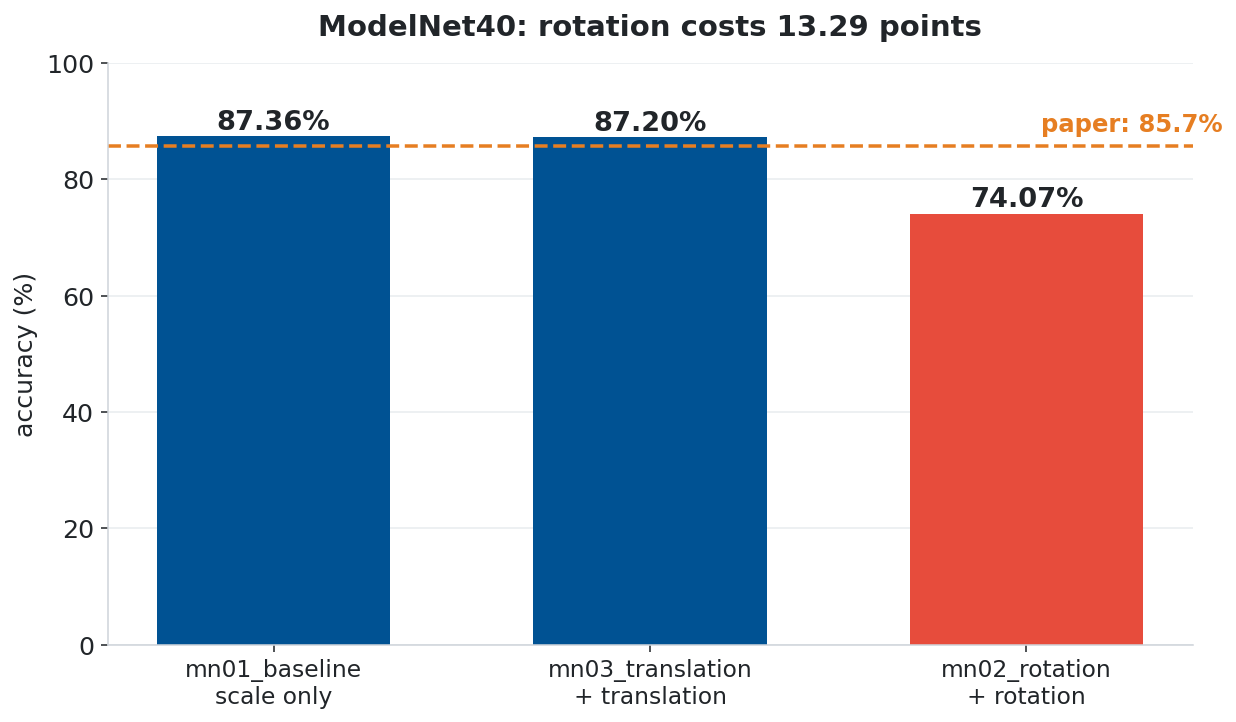
\includegraphics[width=\textwidth,height=0.60\textheight,keepaspectratio]{modelnet40_correct.png}

      \vspace{0.2em}
      \colhead{Above the paper}
        \small
        \textbf{87.36\%} vs the paper's \textbf{85.7\%}, with a batch $16\times$ smaller. Plausible: ModelNet40 is small and its objects arrive canonically aligned, so the large-batch advantage that dominates ImageNet counts for little here.
      
    \end{column}
  \end{columns}
\end{frame}

% ── ModelNet40 augmentation ──────────────────────────────────────────────────
\begin{frame}[shrink=5]{ModelNet40: Rotation Costs 13 Points --- and Why}
  \lead{Translation is free. Rotation costs 13.29 points — and the reason is the positional encoding again.}
  \begin{columns}[T]
    \begin{column}{0.46\textwidth}
      \begin{table}
        \centering\small
        \begin{tabular}{lcc}
          \toprule
          \textbf{Augmentation} & \textbf{Accuracy} & \textbf{$\Delta$} \\
          \midrule
          scale only & \textbf{87.36\%} & --- \\
          $+$ translation & 87.20\% & $-0.16$ \\
          $+$ rotation & \textcolor{AccentRed}{74.07\%} & \textcolor{AccentRed}{\textbf{$-13.29$}} \\
          \bottomrule
        \end{tabular}
      \end{table}

      \vspace{0.4em}
      \colhead{The largest effect in the whole project}
        \small
        And the one with the cleanest theoretical explanation.
      
    \end{column}
    \begin{column}{0.50\textwidth}
      \colhead{The Perceiver has no rotational inductive bias}
        \small
        3D Fourier PE encodes \textbf{absolute} position. Rotating an object changes every coordinate --- and therefore every encoding --- while the label stays the same. The network must learn from scratch an invariance the architecture does not grant, and that this task does not even need: ModelNet40 objects are already canonically aligned.

        \vspace{0.4em}
        Translation is nearly harmless ($-0.16$) because it shifts all points equally: the \emph{relative} structure survives.
      

      \vspace{0.2em}
      \scriptsize \textbf{Takeaway:} a missing inductive bias cannot be patched with augmentation.
    \end{column}
  \end{columns}
\end{frame}

\section{Perceiver IO}

% -- Perceiver IO: Structured Outputs ------------------------------------------------
\begin{frame}[shrink=5]{Perceiver IO: Structured Outputs}
  \begin{center}
    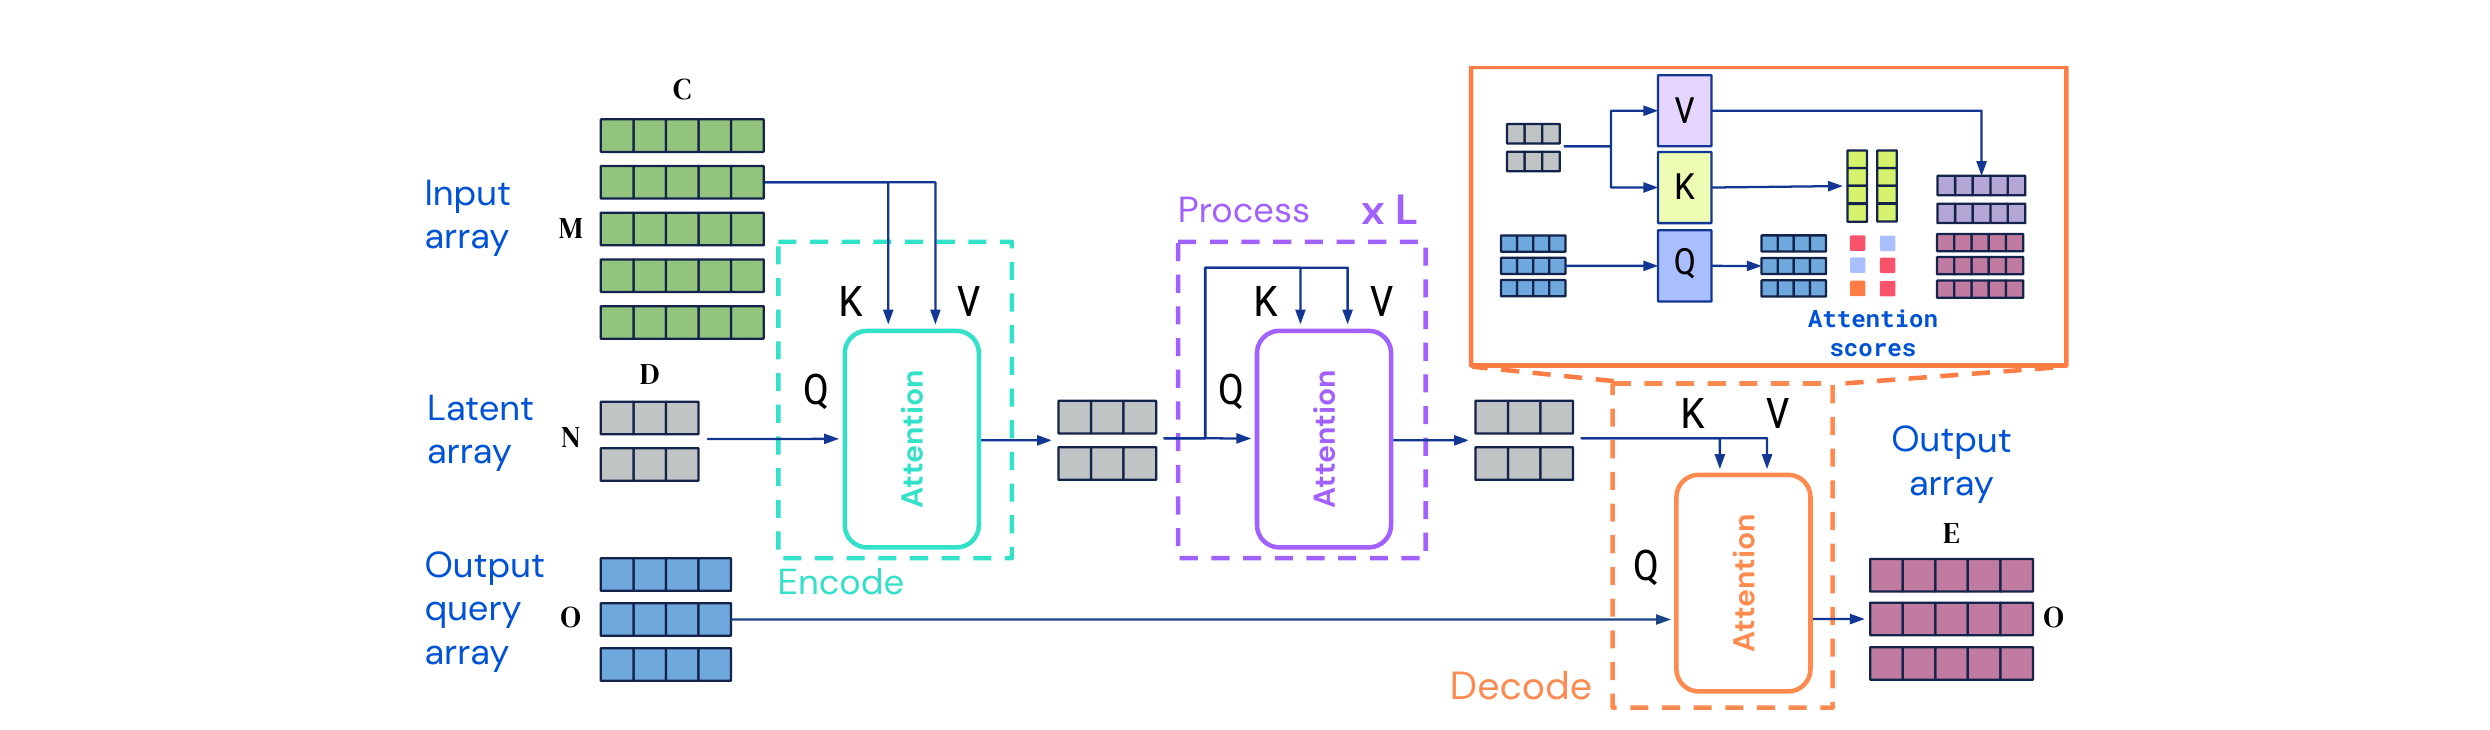
\includegraphics[width=0.95\textwidth,height=0.40\textheight,keepaspectratio]{perceiverio_arch.png}
  \end{center}

  \vspace{0.15em}
  \begin{columns}[T,onlytextwidth]
    \begin{column}{0.48\textwidth}
      \small
      \textbf{Extension over Perceiver} (Jaegle et al., ICLR 2022):
      \begin{itemize}
        \item \textbf{Encode}: input $\rightarrow$ latent (same cross-attn encoder)
        \item \textbf{Process}: latent self-attention ($\times L$)
        \item \textbf{Decode}: \alert{output queries} read latents
      \end{itemize}
    \end{column}
    \begin{column}{0.48\textwidth}
      \small
      \textbf{Why it matters:}
      \begin{itemize}
        \item Original Perceiver: one pooled global output
        \item IO: task-specific output shape
        \item Same latent bottleneck, more general decoder
      \end{itemize}
    \end{column}
  \end{columns}
\end{frame}

% -- Perceiver IO Decoder ------------------------------------------------------------
\begin{frame}[shrink=12]{Perceiver IO Decoder with Output Queries}
  \begin{center}
    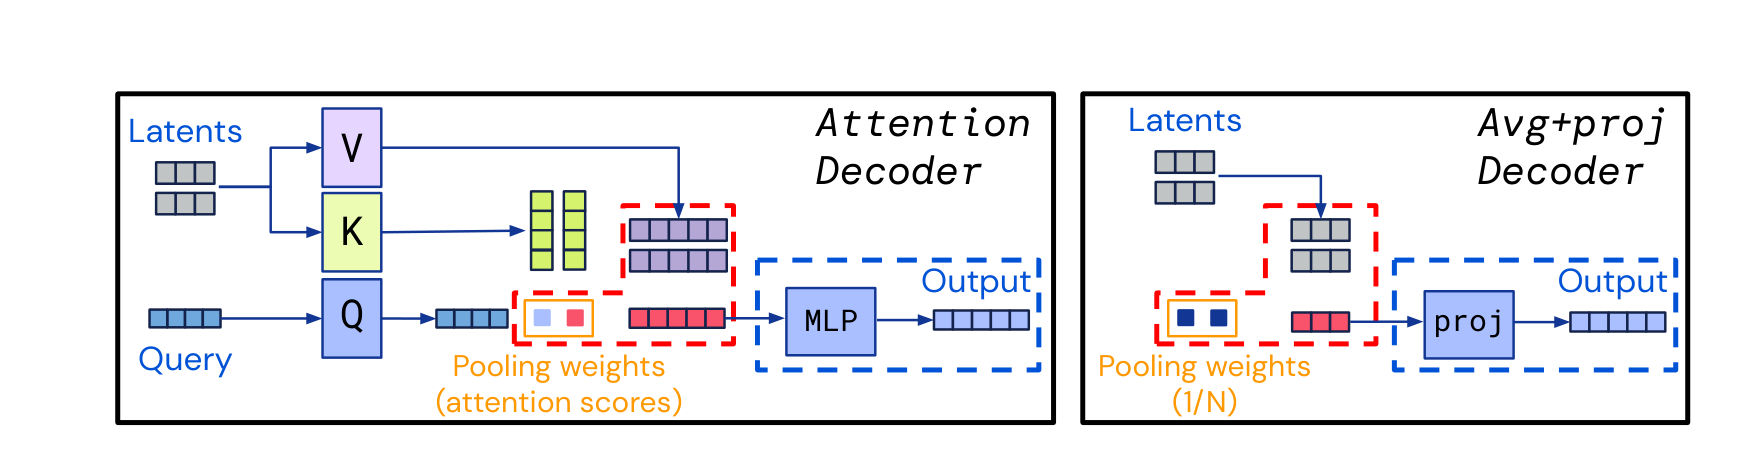
\includegraphics[width=0.86\textwidth,height=0.31\textheight,keepaspectratio]{perceiver_io_decoder.png}
  \end{center}

  \vspace{0.25em}
  \textbf{Decoder cross-attention (single layer):}
  \[
  Q_{\text{dec}} = \text{OutputQuery}\,W_Q, \quad
  K_{\text{dec}} = \text{Latent}\,W_K, \quad
  V_{\text{dec}} = \text{Latent}\,W_V
  \]
  \[
  \text{Output} = \text{softmax}\!\left(\frac{Q_{\text{dec}} K_{\text{dec}}^\top}{\sqrt{d_k}}\right) V_{\text{dec}} \in \mathbb{R}^{O \times D}
  \]

  \vspace{0.3em}
  \begin{itemize}
    \item A task head then projects each of the $O$ rows to the output channels $E$ (logits, pixels, bytes)
    \item The number of output queries $O$ is \textbf{task-dependent} and independent of $N$ and $M$
    \item A single decoder cross-attention layer suffices (no self-attention among outputs)
  \end{itemize}
\end{frame}

% -- Output Query Design -------------------------------------------------------------
\begin{frame}[shrink=4]{Output Query Design per Task}
  \begin{center}
  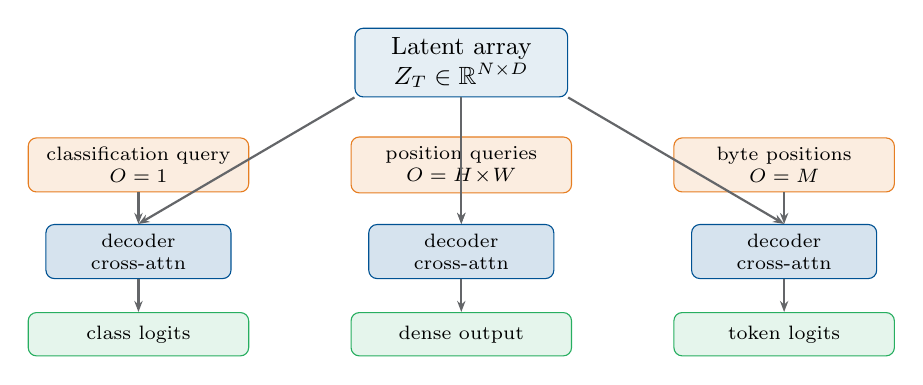
\begin{tikzpicture}[
    latent/.style={rectangle, draw=UnifiBlue, fill=UnifiBlue!10,
                   rounded corners=3pt, minimum width=2.7cm,
                   minimum height=0.62cm, align=center, font=\small},
    query/.style={rectangle, draw=AccentOrange, fill=AccentOrange!14,
                  rounded corners=3pt, minimum width=2.8cm,
                  minimum height=0.55cm, align=center, font=\scriptsize},
    dec/.style={rectangle, draw=UnifiBlue, fill=UnifiBlue!16,
                rounded corners=3pt, minimum width=2.35cm,
                minimum height=0.55cm, align=center, font=\scriptsize},
    outbox/.style={rectangle, draw=AccentGreen, fill=AccentGreen!12,
                   rounded corners=3pt, minimum width=2.8cm,
                   minimum height=0.55cm, align=center, font=\scriptsize},
    arr/.style={-{Stealth[length=4pt]}, thick, UnifiDark!70}
  ]
    \node[latent] (lat) at (0,1.65) {Latent array\\$Z_T \in \mathbb{R}^{N\times D}$};

    \node[query] (q1) at (-4.1,0.35) {classification query\\$O=1$};
    \node[query] (q2) at (0,0.35) {position queries\\$O=H\!\times\!W$};
    \node[query] (q3) at (4.1,0.35) {byte positions\\$O=M$};

    \node[dec] (d1) at (-4.1,-0.75) {decoder\\cross-attn};
    \node[dec] (d2) at (0,-0.75) {decoder\\cross-attn};
    \node[dec] (d3) at (4.1,-0.75) {decoder\\cross-attn};

    \node[outbox] (o1) at (-4.1,-1.80) {class logits};
    \node[outbox] (o2) at (0,-1.80) {dense output};
    \node[outbox] (o3) at (4.1,-1.80) {token logits};

    \draw[arr] (q1) -- (d1);
    \draw[arr] (q2) -- (d2);
    \draw[arr] (q3) -- (d3);
    \draw[arr] (d1) -- (o1);
    \draw[arr] (d2) -- (o2);
    \draw[arr] (d3) -- (o3);
    \draw[arr] (lat.south west) -- (d1.north);
    \draw[arr] (lat.south) -- (d2.north);
    \draw[arr] (lat.south east) -- (d3.north);
  \end{tikzpicture}
  \end{center}

  \vspace{0.2em}
  \begin{columns}[T,onlytextwidth]
    \begin{column}{0.31\textwidth}
      \colhead{Classification}
        \scriptsize One learned query produces one global prediction.
      
    \end{column}
    \begin{column}{0.31\textwidth}
      \colhead{Dense outputs}
        \scriptsize Output shape is controlled by the query array.
      
    \end{column}
    \begin{column}{0.31\textwidth}
      \colhead{Masked LM}
        \scriptsize One query per byte; the loss counts only the masked ones.
      
    \end{column}
  \end{columns}
\end{frame}



\section{Experiments: Perceiver IO}

% -- CIFAR comparison after IO explanation ------------------------------------------
\begin{frame}[shrink=20]{Perceiver IO on CIFAR-10: the Decoder Changes Nothing Here}
  \lead{On a single label out of ten, the query decoder and mean pooling are the same thing — and the measurement says so.}
  \begin{columns}[T,onlytextwidth]
    \begin{column}{0.56\textwidth}
      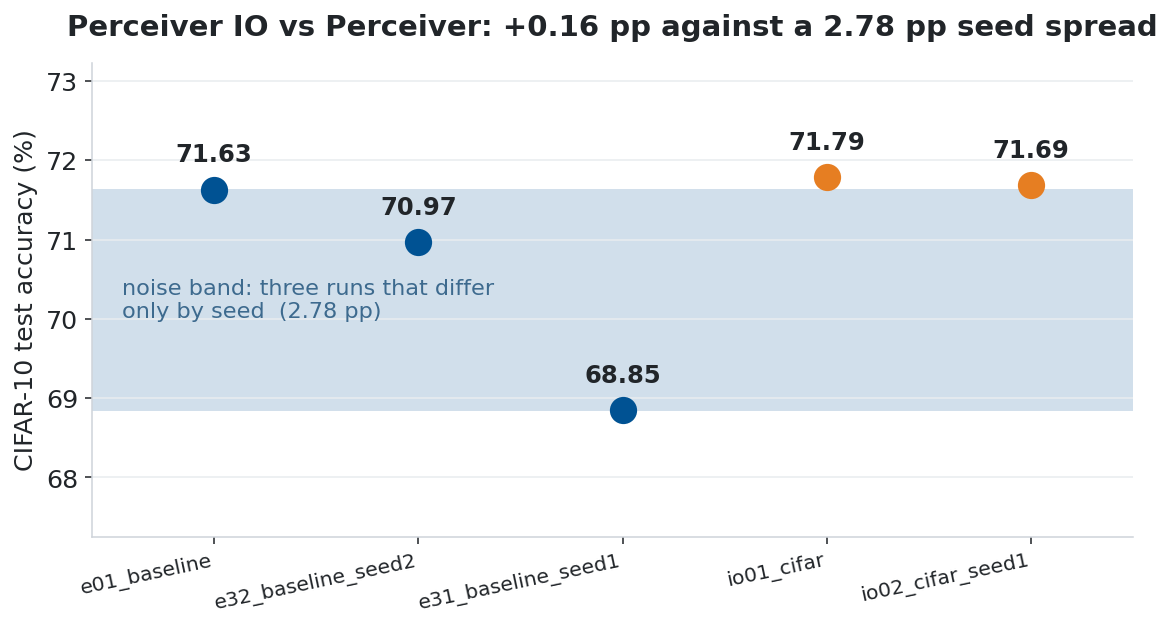
\includegraphics[width=\textwidth,height=0.62\textheight,keepaspectratio]{perceiver_vs_io_correct.png}
    \end{column}
    \begin{column}{0.40\textwidth}
      \colhead{What changed, and what did not}
        \small
        Same encoder as \texttt{e01\_baseline}; the mean-pooling head is replaced by a \textbf{decoder with one output query}, and the training recipe follows the IO paper (App.~A.1): lr $10^{-3}$, cosine.

        \vspace{0.3em}
        \texttt{io01\_cifar} \textbf{71.79\%} vs \texttt{e01} \textbf{71.63\%}: $+0.16$pp, against a seed spread of \textbf{2.78pp}. The replica \texttt{io02} lands at 71.69\%.
      

      \vspace{0.3em}
      \colhead{This was the expected outcome}
        \small
        \alert{No difference is the result}, not a disappointment. The decoder earns its keep when the output is \textbf{structured} --- one query per byte in the MLM, one per task in the multitask run. For one label out of ten, querying the latents and averaging them are the same thing.
      
    \end{column}
  \end{columns}
\end{frame}

% ── MLM ──────────────────────────────────────────────────────────────────────
\begin{frame}[shrink=12]{WikiText-103: Byte-Level Masked Language Model}
  \lead{Pre-train a language encoder with no tokenizer at all: the input is the raw UTF-8 byte stream.}
  \begin{columns}[T]
    \begin{column}{0.46\textwidth}
      \begin{table}
        \centering\small
        \begin{tabular}{ll}
          \toprule
          \textbf{Setting} & \textbf{Value} \\
          \midrule
          Latent array & $128 \times 512$ \\
          Cross-attn / blocks & 1 / 4 \\
          Heads (cross / self) & 1 / 8 \\
          Sequence length & 512 bytes \\
          Vocabulary & $256 + 1$ mask \\
          Masking rate & 15\% \\
          Output queries & one per position \\
          Optimizer / lr & LAMB / 0.001 \\
          Epochs / batch & 10 / 32 \\
          Parameters & 18\,872\,740 \\
          \midrule
          \textbf{Masked-byte accuracy} & \textbf{86.68\%} \\
          Chance level ($1/256$) & 0.39\% \\
          \bottomrule
        \end{tabular}
      \end{table}
    \end{column}
    \begin{column}{0.50\textwidth}
      \colhead{Where the decoder finally earns its keep}
        \small
        \textbf{$\sim$222$\times$ better than chance}, reading raw UTF-8 with \textbf{no tokenizer at all}. Nearly nine masked bytes out of ten reconstructed.
      

      \vspace{0.3em}
      \colhead{Why bytes are affordable here}
        \small
        Cross-attention costs $O(M \cdot N)$ --- \emph{linear} in sequence length --- instead of $O(M^2)$. Going from 512 tokens to 2\,048 bytes costs BERT $16\times$ in attention, and Perceiver IO only $4\times$.
      

      \vspace{0.3em}
      \alerthead{Read this number carefully}
        \scriptsize
        Masked-\emph{byte} accuracy is not comparable to masked-\emph{token} accuracy: the space is 256, not tens of thousands. It shows the pre-training worked --- the comparison with BERT lives on GLUE.
      
    \end{column}
  \end{columns}
\end{frame}

% ── GLUE ─────────────────────────────────────────────────────────────────────
\begin{frame}[shrink=11]{GLUE: Eight Tasks, One Encoder, No Tokenizer}
  \lead{The same encoder, the same weights, one query swapped — and two of the eight numbers turn out not to be learning.}
  \begin{columns}[T,onlytextwidth]
    \begin{column}{0.52\textwidth}
      \begin{table}
        \centering\scriptsize
        \begin{tabular}{llcc}
          \toprule
          \textbf{Run} & \textbf{Task} & \textbf{Budget} & \textbf{Result} \\
          \midrule
          \texttt{io\_glue\_cola} & acceptability & 30 & \textcolor{gray}{69.13} \\
          \texttt{io\_glue\_sst2} & sentiment & 10 & 80.73 \\
          \texttt{io\_glue\_mrpc} & paraphrase & 30 & \textcolor{gray}{70.59} \\
          \texttt{io\_glue\_stsb} & similarity (reg.) & 30 & 60.82 \\
          \texttt{io\_glue\_qqp} & duplicate Q & 3 & \textbf{84.66} \\
          \texttt{io\_glue\_mnli} & NLI (3-way) & 3 & 65.80 \\
          \texttt{io\_glue\_qnli} & QA entailment & 10 & 80.65 \\
          \texttt{io\_glue\_rte} & entailment & 30 & 56.68 \\
          \midrule
          \multicolumn{3}{l}{\textbf{Mean over the eight}} & \textbf{71.13} \\
          \multicolumn{3}{l}{\textit{Paper, Tab. 1 (byte-level)}} & \textit{81.0} \\
          \bottomrule
        \end{tabular}
      \end{table}
      \scriptsize STS-B is Pearson $\times 100$, the official GLUE metric. \textcolor{gray}{Grey} marks the two majority-class predictors. Fine-tuning starts from the MLM checkpoint; the epoch budget follows task size (393\,k examples against 2.5\,k).
    \end{column}
    \begin{column}{0.44\textwidth}
      \alerthead{Two of these numbers are not learning}
        \small
        \textbf{CoLA} scores 721 correct out of 1\,043 --- \emph{exactly} the majority-class count. \textbf{MRPC} beats its majority by 9 examples out of 408. Both are constant predictors wearing an accuracy.

        \vspace{0.3em}
        The mean of 71.13 therefore rests on \textbf{six} tasks, not eight. CoLA in the paper is scored with Matthews' correlation, which for a constant predictor is \textbf{0}.
      

      \vspace{0.3em}
      \colhead{The gap that does not close}
        \small
        71.13 against the paper's 81.0. The scale is not comparable: \textbf{18.9M} parameters pre-trained on WikiText-103 for 10 epochs, against \textbf{201M} on Wikipedia $+$ C4 for 500\,000 steps.
      
    \end{column}
  \end{columns}
\end{frame}

% ── GLUE: quanto vale il pre-training ────────────────────────────────────────
\begin{frame}[shrink=11]{GLUE: What the Pre-training Is Actually Worth}
  \lead{Two tasks fine-tuned twice — once from the MLM checkpoint, once from random weights. Everything else identical.}
  \begin{columns}[T,onlytextwidth]
    \begin{column}{0.50\textwidth}
      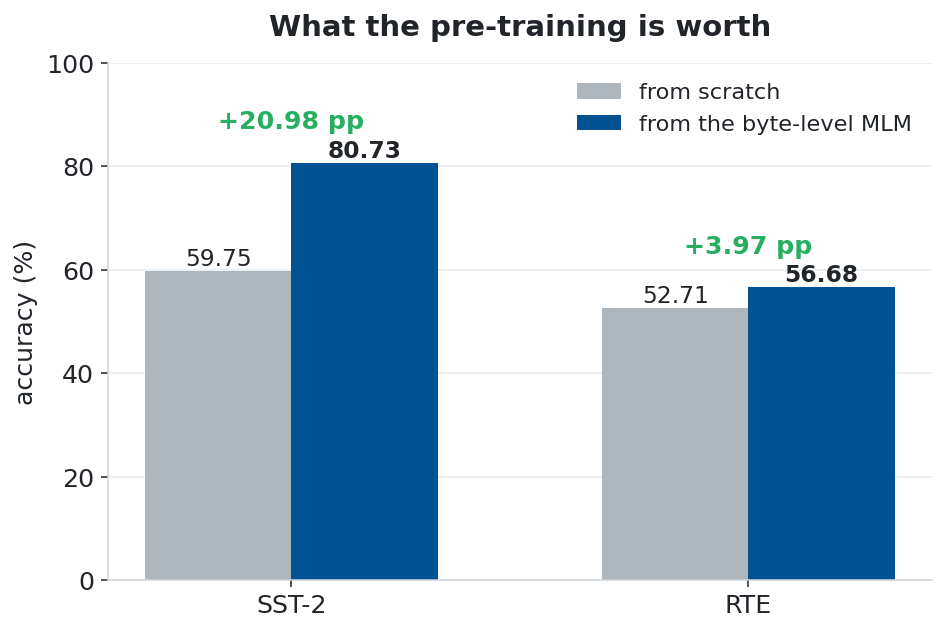
\includegraphics[width=\textwidth,height=0.62\textheight,keepaspectratio]{pretraining_value_correct.png}
    \end{column}
    \begin{column}{0.46\textwidth}
      \colhead{Why two controls and not eight}
        \small
        A fine-tuned 80\% means nothing on its own --- maybe the task is solvable at 80\% from random weights. The two \texttt{scratch} runs are chosen at the \textbf{extremes} of data size: \textbf{SST-2} has 67\,000 training examples, \textbf{RTE} has 2\,500. Everything else is identical.
      

      \vspace{0.3em}
      \colhead{And the prediction holds}
        \small
        SST-2: $59.75\% \to \mathbf{80.73\%}$, \textcolor{AccentGreen}{\textbf{$+$20.98pp}}.\
        RTE: $52.71\% \to \mathbf{56.68\%}$, \textcolor{AccentGreen}{\textbf{$+$3.97pp}}.

        \vspace{0.3em}
        Transfer is worth five times more where the data abounds. The small task cannot exploit the encoder it was given: 2\,500 examples are not enough to move it far from its starting point.
      
    \end{column}
  \end{columns}
\end{frame}

% ── GLUE multitask (paper IO, Tab. 2) ────────────────────────────────────────
\begin{frame}[shrink=14]{GLUE Multitask: the Comparison That Replicates Best}
  \lead{One model with eight output queries against eight separate fine-tunings — the comparison from Table 2 of the IO paper.}
  \begin{columns}[T,onlytextwidth]
    \begin{column}{0.56\textwidth}
      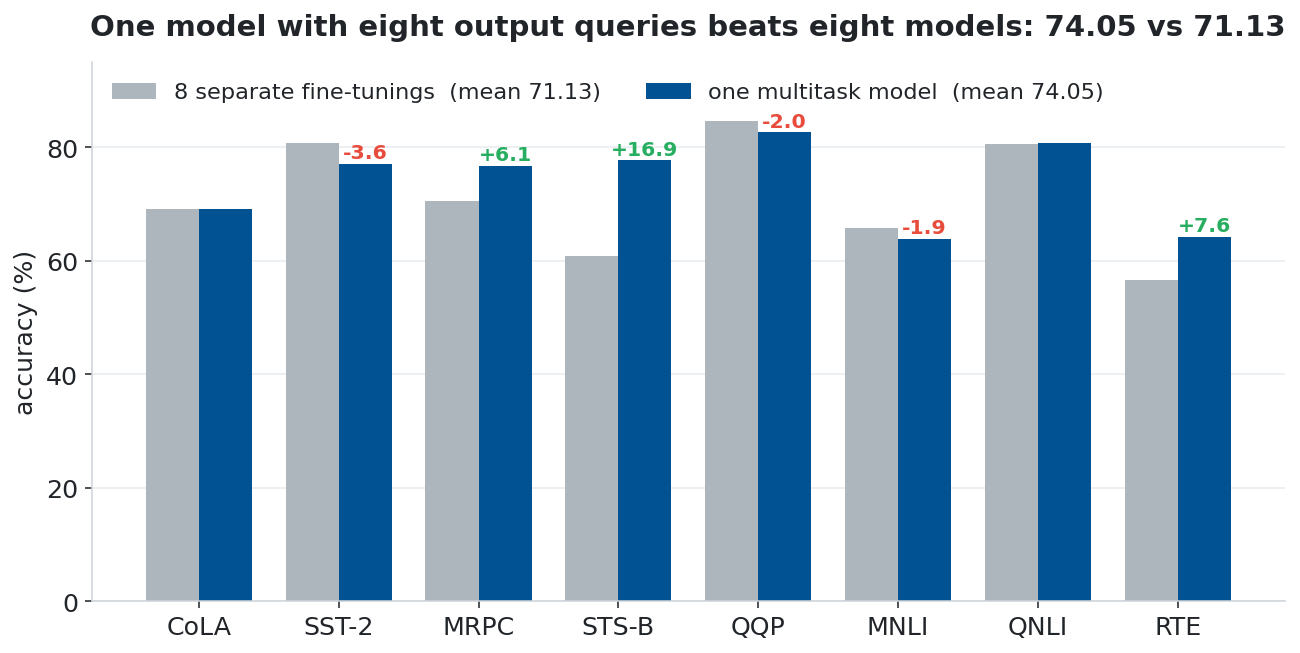
\includegraphics[width=\textwidth,height=0.60\textheight,keepaspectratio]{multitask_glue_correct.png}
    \end{column}
    \begin{column}{0.40\textwidth}
      \colhead{Table 2 of the IO paper}
        \small
        One model with \textbf{one output query per task}, against eight separate fine-tunings. Paper: $81.8$ vs $81.0$, \textbf{$+0.8$}. Here: 74.05 vs 71.13, \textcolor{AccentGreen}{\textbf{$+$2.92}}.

        \vspace{0.3em}
        The absolute level stays $\sim$8 points below. But \textbf{sign and order of magnitude hold} --- and that relation, not the level, is what Tab.~2 claims.
      

      \vspace{0.3em}
      \colhead{Not a fair fight --- in our favour}
        \small
        The multitask model selects \textbf{one} epoch for all eight tasks; the separate models select \textbf{eight}. It wins anyway --- and a ninth task would cost \textbf{one query}, not another model.
      
    \end{column}
  \end{columns}
\end{frame}

\begin{frame}[shrink=17]{Convergence: When Each Run Peaks}
  \lead{There is no early stopping: every run trains the full schedule and reports the checkpoint that was best on validation.}
  \begin{columns}[T]
    \begin{column}{0.58\textwidth}
      \begin{center}
        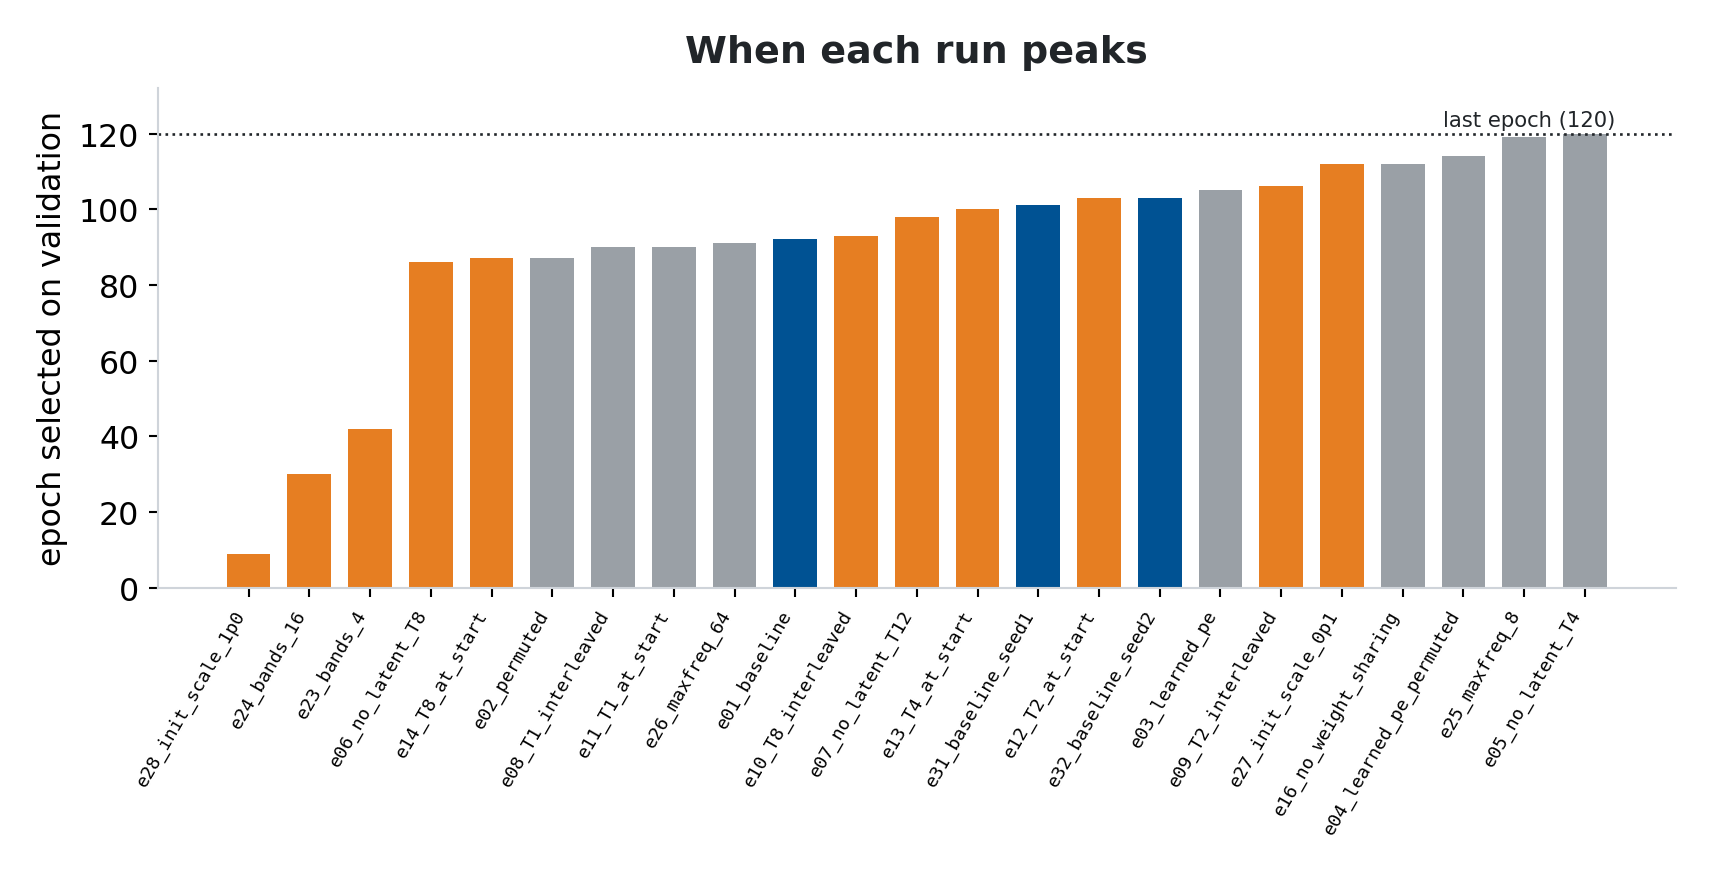
\includegraphics[width=\textwidth,height=0.60\textheight,keepaspectratio]{convergence_epochs_correct.png}
      \end{center}
    \end{column}
    \begin{column}{0.38\textwidth}
      \textbf{Why this matters}

      \vspace{0.3em}
      The distribution of best epochs is itself a diagnostic: a run that peaks early and then decays is unstable, whatever its best number says.

      \vspace{0.5em}
      \alerthead{Three unstable runs}
        \small
        Validation accuracy, best epoch $\to$ final epoch:\\
        \texttt{e23}: 67.74\% @42 $\to$ \textbf{22.54\%}\\
        \texttt{e24}: 62.66\% @30 $\to$ \textbf{55.46\%}\\
        \texttt{e28}: 53.36\% @\textbf{9} $\to$ 46.32\%

        \vspace{0.3em}
        \scriptsize Their reported numbers come from the validation-selected checkpoint --- the correct methodology --- but the instability has to be declared, not hidden.
      

      \vspace{0.3em}
      \scriptsize \texttt{e05\_no\_latent\_T4} peaks at epoch \textbf{120}: it was still improving when the schedule ended.
    \end{column}
  \end{columns}
\end{frame}

% ── Slide 27: Attention Maps ────────────────────────────────────────────────────
\begin{frame}[shrink=8]{Attention Maps: Where the Latents Look}
  \lead{With coordinates the latents pick locations; without, they can only pick colours.}
  \begin{center}
    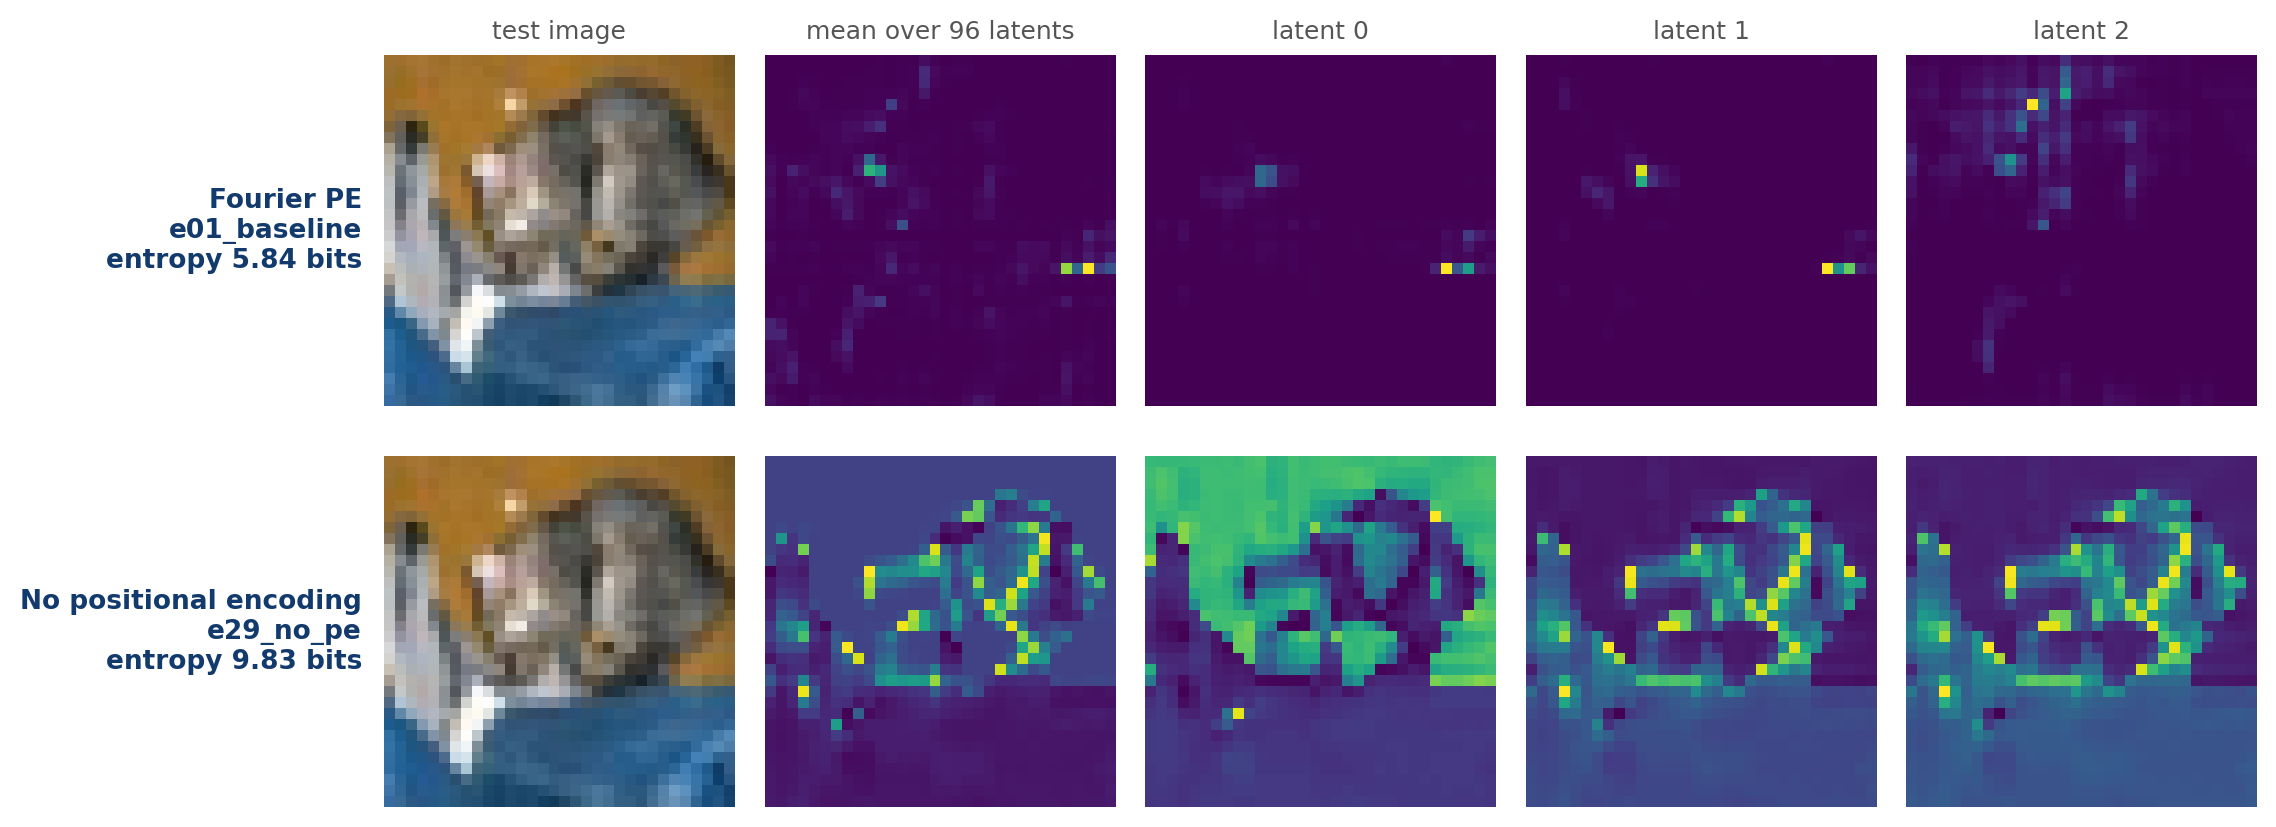
\includegraphics[width=0.98\textwidth,height=4.0cm,keepaspectratio]{attention_maps_v2.png}
  \end{center}

  \vspace{0.1em}
  \begin{columns}[T,onlytextwidth]
    \begin{column}{0.48\textwidth}
      \colhead{Fourier PE (\texttt{e01}, 71.63\%)}
        \small Each latent attends to a few pixels at specific locations: mean entropy \textbf{5.84 bits} over 1\,024 pixels (uniform: 10 bits). Latents specialise by region.
    \end{column}
    \begin{column}{0.48\textwidth}
      \alerthead{No PE (\texttt{e29}, 32.36\%)}
        \small Same-colour pixels are indistinguishable: attention follows colour boundaries and spreads over the image --- \textbf{9.83 bits}, 98\% of uniform.
    \end{column}
  \end{columns}
\end{frame}

% ── Slide 28: Comprehensive Results Summary ─────────────────────────────────────
\begin{frame}[shrink=28]{Comprehensive Results Summary}
  \lead{Forty-two runs, all completed. Every number below traces to a results.json — none is quoted from memory.}
  \begin{table}
    \centering\small
    \begin{tabular}{llccl}
      \toprule
      \textbf{Modality} & \textbf{Model} & \textbf{Best Acc.} & \textbf{Reference} & \textbf{Experiments} \\
      \midrule
      Images (CIFAR-10) & Perceiver & 72.91\% & 93.61\%$^{\dagger}$ & \textbf{24} runs \\
      Images (CIFAR-10) & Perceiver IO & 71.79\% & 71.63\% (Perceiver) & 2 \\
      Point Clouds (ModelNet40) & Perceiver & \textbf{87.36\%} & 85.7\% & 3 augmentations \\
      Text (WikiText-103) & Perceiver IO & \textbf{86.68\%} MLM & 0.39\% chance & 1 \\
      NLU (GLUE, 8 tasks) & Perceiver IO & 71.13 mean & 81.0 (paper) & 11 \\
      Images (CIFAR-10) & ResNet-18 & \textbf{93.61\%} & --- & 1 \\
      \bottomrule
    \end{tabular}
  \end{table}

  {\scriptsize $^{\dagger}$ A ResNet-18 trained here under identical conditions. Neither Perceiver paper benchmarks CIFAR-10, so the reference had to be measured rather than quoted.}

  \vspace{0.4em}
  \begin{columns}[T]
    \begin{column}{0.48\textwidth}
      \textbf{What is measured}
      \begin{itemize}\small
        \item ModelNet40 \textbf{beats} the paper: $+$1.66pp
        \item Byte-level MLM works: 86.68\% against a 0.39\% chance level
        \item One multitask model beats eight separate ones: 74.05 vs 71.13
        \item Noise band \textbf{2.78pp}, measured on 3 seed replicas
        \item 12 of 24 CIFAR runs are conclusive
      \end{itemize}
    \end{column}
    \begin{column}{0.48\textwidth}
      \textbf{Scope of the campaign}
      \begin{itemize}\small
        \item Declarative registry of \textbf{42 runs}, \textbf{42} completed
        \item 3 modalities: 2D images, 3D point clouds, raw bytes
        \item One command per run: \texttt{experiments.py --run <id>}
        \item Every figure above traces to a \texttt{results.json}; none is quoted from memory
      \end{itemize}
    \end{column}
  \end{columns}
\end{frame}

% ══════════════════════════════════════════════════════════════════════════════
% SECTION 4: Criticalities & Discussion (slides 29-33)
% ══════════════════════════════════════════════════════════════════════════════
\section{Conclusion}

% ── Slide 29: Gap vs Original Paper ─────────────────────────────────────────────
\begin{frame}[shrink=22]{Gap vs Original Papers}
  \lead{On the modality with the weakest domain prior we beat the paper. On the one with the strongest, a convolutional net of the same size beats us.}
  \begin{columns}[T]
    \begin{column}{0.48\textwidth}
      \textbf{ModelNet40 (Point Clouds):}
      \begin{table}
        \centering\small
        \begin{tabular}{lc}
          \toprule
          \textbf{Source} & \textbf{Acc.} \\
          \midrule
          Original Paper & 85.7\% \\
          This implementation & \textbf{87.36\%} \\
          \midrule
          \textbf{Gap} & \textcolor{AccentGreen}{\textbf{$+$1.66pp}} \\
          \bottomrule
        \end{tabular}
      \end{table}

      \vspace{0.3em}
      \textbf{We are above the paper.}\\
      With a batch $16\times$ smaller (32 vs 512). Plausible because ModelNet40 is small and canonically aligned, so the large-batch advantage counts for little.
    \end{column}
    \begin{column}{0.48\textwidth}
      \textbf{CIFAR-10 (Images):}
      \begin{table}
        \centering\small
        \begin{tabular}{lc}
          \toprule
          \textbf{Source} & \textbf{Acc.} \\
          \midrule
          ResNet-18, same budget & \textbf{93.61\%} \\
          \texttt{e01\_baseline} & 71.63\% \\
          \midrule
          \textbf{Gap} & \textcolor{AccentRed}{\textbf{$-$21.98pp}} \\
          \bottomrule
        \end{tabular}
      \end{table}

      \vspace{0.3em}
      \textbf{The reference had to be measured.}\\
      Neither Perceiver paper benchmarks CIFAR-10, so a convolutional net was trained here under identical conditions rather than quoting a number from elsewhere.
    \end{column}
  \end{columns}

  \vspace{0.5em}
  \colhead{What the two columns say together}
    On the modality with a \textbf{weak} domain prior --- 3D point clouds --- we are above the paper. On the one with a \textbf{strong} prior, a convolutional net of the same size wins by 22 points. On ImageNet the paper beats ResNet-50 by $+4.5$pp: the prior stops paying at scale, and \alert{that is the claim being replicated}, not an absolute accuracy.
  
\end{frame}

% ── Slide 30: Hardware Limitations ──────────────────────────────────────────────
\begin{frame}[shrink=14]{Hardware Limitations \& Design Choices}
  \lead{Every limitation below is one GPU instead of 512 TPU cores. The architecture is the paper's; the budget is not.}
  \begin{table}
    \centering\small
    \begin{tabular}{lcc}
      \toprule
      \textbf{Parameter} & \textbf{Original Paper (Google)} & \textbf{Project Setup} \\
      \midrule
      Hardware & 512 TPU v3 cores & 1 NVIDIA RTX 3080 \\
      Batch size & up to 1024 & 32--64 \\
      Latents ($N$) & 256--512 & 96--128 \\
      Model size & 30--200M+ params & 10.2--23.3M params \\
      Pre-training corpus & Wikipedia $+$ C4, 201M-param IO & WikiText-103, 18.9M-param IO \\
      \bottomrule
    \end{tabular}
  \end{table}

  \vspace{0.5em}
  \begin{columns}[T]
    \begin{column}{0.48\textwidth}
      \textbf{Consequences:}
      \begin{itemize}
        \item LAMB at batch 32--64, not the 512--1024 it targets
        \item 96--128 latents instead of 512
        \item One seed per ablation, three for the baseline
        \item No search beyond the registered ablations
      \end{itemize}
    \end{column}
    \begin{column}{0.48\textwidth}
      \textbf{Mitigation strategies:}
      \begin{itemize}
        \item Weight sharing: 10.2M parameters, not 31.5M
        \item bf16 autocast $+$ gradient clipping (LAMB at lr 0.004)
        \item A measured noise band, not more runs per cell
        \item Validation carved from train; test touched once
      \end{itemize}
    \end{column}
  \end{columns}
\end{frame}

% ── Slide 31: Possible Improvements ─────────────────────────────────────────────
\begin{frame}[shrink=9]{Possible Improvements}
  \begin{columns}[T]
    \begin{column}{0.48\textwidth}
      \textbf{Architecture:}
      \begin{itemize}
        \item Increase latent count ($N = 256$+) with gradient checkpointing
        \item Add multi-scale cross-attention (coarse $\rightarrow$ fine)
        \item Explore relative positional encodings (RoPE, ALiBi)
        \item Deeper decoder for structured outputs
      \end{itemize}

      \vspace{0.5em}
      \textbf{Training:}
      \begin{itemize}
        \item Larger batch sizes with gradient accumulation
        \item More seeds per ablation, to narrow the 2.78pp band
        \item Longer training schedules
        \item Advanced augmentation (CutMix, MixUp)
      \end{itemize}
    \end{column}
    \begin{column}{0.48\textwidth}
      \textbf{Data \& Tasks:}
      \begin{itemize}
        \item ImageNet pre-training for vision
        \item Longer byte-level pre-training: more epochs, larger corpus
        \item Multi-modal joint training
        \item Audio modality experiments
      \end{itemize}

      \vspace{0.5em}
      \textbf{Analysis:}
      \begin{itemize}
        \item Layer-wise attention probing
        \item Latent space clustering visualization
        \item Systematic hyperparameter search
        \item Comparison with efficient Transformers (Linformer, Performer)
      \end{itemize}
    \end{column}
  \end{columns}
\end{frame}

% ── Slide 32: Lessons Learned ───────────────────────────────────────────────────
\begin{frame}[shrink=17]{Empirical Summary}
  \lead{Everything measured, split by whether it survived the noise band.}
  \begin{columns}[T]
    \begin{column}{0.48\textwidth}
      \textbf{Conclusive (outside the 2.78pp band):}
      \begin{itemize}\small
        \item \textbf{Positional encoding} is the whole thing: removing it costs \textbf{39.27pp} (71.63$\to$32.36\%)
        \item \textbf{Generality}: one architecture, 87.36\% on 3D point clouds --- above the paper --- and 86.68\% on raw bytes
        \item \textbf{Pre-training transfers}: SST-2 59.75$\to$80.73\%, and 5$\times$ less on the small task
        \item \textbf{Latent init scale} is the critical hyperparameter: 0.02$\to$71.63\%, 1.0$\to$52.08\%
        \item \textbf{Interleaving} cross-attends beats front-loading by 4.44pp
        \item \textbf{Rotation augmentation} costs 13.29pp on ModelNet40
      \end{itemize}
    \end{column}
    \begin{column}{0.48\textwidth}
      \textbf{Inside the band --- ``no measurable damage'':}
      \begin{itemize}\small
        \item Permutation invariance, with \emph{both} positional encodings
        \item Weight sharing: $3.1\times$ fewer parameters at no measurable cost
        \item Perceiver IO vs Perceiver on images: $+0.16$pp
      \end{itemize}

      \vspace{0.4em}
      \textbf{Measured, and not in our favour:}
      \begin{itemize}\small
        \item A ResNet-18 on the same budget: \textbf{93.61\%} vs 71.63\%
        \item GLUE mean 71.13 against the paper's 81.0
        \item Two GLUE tasks (CoLA, MRPC) are majority-class predictors
        \item No configuration beats the baseline outside the band --- every conclusive effect is \textbf{negative}
      \end{itemize}
    \end{column}
  \end{columns}

  \vspace{0.5em}
  \colhead{Central methodological finding}
    Measuring the \textbf{noise band} --- three replicas differing only by seed --- cost two runs and changed the status of all the others. Without it, 12 of the 24 comparisons would have been reported as effects when they are variance.
  
\end{frame}

% ── Slide 33: Conclusions ───────────────────────────────────────────────────────
\begin{frame}[shrink=21]{Conclusions}
  \lead{What the architecture gives, and what it still costs at this scale.}
  \begin{columns}[T]
    \begin{column}{0.48\textwidth}
      \textbf{Architecture properties:}
      \begin{itemize}
        \item Single architecture for images, point clouds, and text
        \item Linear complexity in input size
        \item Weight sharing: $3.1\times$ fewer parameters at no measurable cost
        \item Zero CNN/RNN domain-specific assumptions
        \item Output queries: one more task costs \textbf{one query}, not another model
      \end{itemize}
    \end{column}
    \begin{column}{0.48\textwidth}
      \textbf{Remaining limitations:}
      \begin{itemize}
        \item At this scale the domain prior is worth \textbf{22 points} (93.61 vs 71.63)
        \item Entirely dependent on the positional encoding ($-$39.27pp without it)
        \item GLUE sits $\sim$10 points below the paper (71.1 vs 81.0), at 1/10 of the parameters and pre-training
        \item LAMB at batch 64 is sensitive to the latent init scale
        \item Half the image ablations are indistinguishable from noise
      \end{itemize}
    \end{column}
  \end{columns}

  \vspace{0.5em}
  \greenhead{Closing statement}
    A \textbf{single general-purpose architecture} does apply to images, point clouds and raw bytes --- and on the modality with the weakest domain prior it beats the paper. Its advantage was never accuracy: it is \alert{having no prior on the domain}. At CIFAR-10 scale that prior is worth 22 points; the paper's own claim is that it stops paying at ImageNet scale, and nothing measured here contradicts it.
  
\end{frame}

% ══════════════════════════════════════════════════════════════════════════════
% SECTION 5: Closing (slides 34-36)
% ══════════════════════════════════════════════════════════════════════════════
% Closing materials: references and appendix.

% ── Slide 35: Appendix – Expected Questions ─────────────────────────────────────
% (References and Expected-Questions slides removed)

% ── Slide 36: Thank You ─────────────────────────────────────────────────────────
\begin{frame}
  \begin{center}
    {\Huge\color{UnifiBlue}\textbf{Thank you!}}\\[1.5em]
    {\Large\color{UnifiDark} Questions?}\\[2.5em]
    {\color{UnifiDark}Francesco Gigli and Corso Vignoli}\\[0.3em]
    {\small\color{UnifiDark} Code and reproduction instructions shared with the course}
  \end{center}
\end{frame}

\end{document}
